\documentclass[11pt]{article}

% Lecture notes template
\usepackage[margin=1in]{geometry}
\usepackage[T1]{fontenc}
\usepackage{lmodern}
\usepackage{amsmath,amssymb,amsthm}
\usepackage{graphicx}
\usepackage{enumitem}
\usepackage{hyperref}
\usepackage{xcolor}
\usepackage{tikz}
\usetikzlibrary{arrows.meta}
\usepackage{listings}

% Python code in the programming exercises.
\lstset{
    language=Python,
    basicstyle=\ttfamily\small,
    keywordstyle=\color{blue!70!black},
    commentstyle=\color{gray!70!black}\itshape,
    stringstyle=\color{orange!70!black},
    showstringspaces=false,
    upquote=true,
    columns=fullflexible,
    keepspaces=true,
    frame=single,
    rulecolor=\color{gray!40},
    backgroundcolor=\color{gray!6},
    xleftmargin=0.5em,
    xrightmargin=0.5em,
}
% Inline Python code, e.g. \py{np.linalg.solve(A, b)}; unlike \lstinline, it can break at spaces.
\newcommand{\py}[1]{\texttt{\detokenize{#1}}}

% Norms and inner products.
\newcommand{\norm}[1]{\lVert #1 \rVert}
\newcommand{\ip}[2]{\langle #1, #2 \rangle}

\title{Lecture 2: Analytic Geometry}
\author{Math for Machine Learning}
\date{\today}

\theoremstyle{definition}
\newtheorem{definition}{Definition}[section]
\newtheorem{example}[definition]{Example}
\newtheorem{exercise}[definition]{Exercise}
\theoremstyle{plain}
\newtheorem{theorem}[definition]{Theorem}
\newtheorem{proposition}[definition]{Proposition}
\newtheorem{lemma}[definition]{Lemma}
\newtheorem{corollary}[definition]{Corollary}
\theoremstyle{remark}
\newtheorem{remark}[definition]{Remark}

\DeclareMathOperator{\im}{im}
\DeclareMathOperator{\rank}{rank}
\DeclareMathOperator{\Null}{null}
\DeclareMathOperator{\col}{col}
\DeclareMathOperator{\row}{row}
\DeclareMathOperator{\Span}{span}
\DeclareMathOperator{\tr}{tr}
\DeclareMathOperator{\diag}{diag}
\DeclareMathOperator{\sign}{sign}

\begin{document}

\maketitle
\tableofcontents

\section*{Introduction}
\addcontentsline{toc}{section}{Introduction}

In Lecture~1, we studied vector spaces and linear transformations. Vector spaces let us add vectors and multiply them by scalars, but they do not tell us how long a vector is, how far apart two vectors are, or what the angle between two vectors is. These geometric notions are essential in machine learning:
\begin{itemize}
    \item data points are vectors, and many algorithms, such as $k$-nearest neighbors and clustering, rely on distances between them;
    \item similarity between data points, such as text documents or word embeddings, is often measured by the angle between vectors;
    \item linear regression and principal component analysis find the orthogonal projection of data onto a subspace;
    \item regularization penalizes the size, i.e., the norm, of a weight vector.
\end{itemize}
In this lecture, we add geometry to vector spaces, using norms and inner products.

Throughout this lecture, all vector spaces are real vector spaces, i.e., vector spaces over $\mathbb{R}$. As in Lecture~1, we write vectors of $\mathbb{R}^n$ as columns, and we identify a $1 \times 1$ matrix with its only entry. In particular, for $x, y \in \mathbb{R}^n$,
\[x^\top y = x_1 y_1 + x_2 y_2 + \cdots + x_n y_n.\]

\section{Norms}

The length of a vector is measured by a norm. There are many reasonable ways to measure length, so we first collect the properties that every notion of length should have.

\begin{definition}[Norm]\label{def:norm}
    A norm on a vector space $V$ is a function $\norm{\cdot}: V \to \mathbb{R}$, $v \mapsto \norm{v}$, such that for all $u, v \in V$ and all $\lambda \in \mathbb{R}$:
    \begin{enumerate}
        \item Positive definiteness: $\norm{v} \geq 0$, and $\norm{v} = 0$ if and only if $v = 0$;
        \item Absolute homogeneity: $\norm{\lambda v} = |\lambda| \, \norm{v}$;
        \item Triangle inequality: $\norm{u + v} \leq \norm{u} + \norm{v}$.
    \end{enumerate}
    A vector space together with a norm is called a normed vector space, or normed space.
\end{definition}

The triangle inequality says that in a triangle with sides $u$, $v$ and $u + v$, the length of one side is at most the sum of the lengths of the other two sides.

\begin{definition}[$\ell_1$, $\ell_2$ and $\ell_\infty$ norms]\label{def:lp}
    For $x = (x_1, \ldots, x_n)^\top \in \mathbb{R}^n$, we define
    \begin{align*}
        \norm{x}_1 &= |x_1| + |x_2| + \cdots + |x_n| && \text{(the $\ell_1$ norm, or Manhattan norm)}, \\
        \norm{x}_2 &= \sqrt{x_1^2 + x_2^2 + \cdots + x_n^2} = \sqrt{x^\top x} && \text{(the $\ell_2$ norm, or Euclidean norm)}, \\
        \norm{x}_\infty &= \max\{|x_1|, |x_2|, \ldots, |x_n|\} && \text{(the $\ell_\infty$ norm, or maximum norm)}.
    \end{align*}
    More generally, for every real number $p \geq 1$, the $\ell_p$ norm is $\norm{x}_p = \big(|x_1|^p + \cdots + |x_n|^p\big)^{1/p}$.
\end{definition}

The name ``Manhattan norm'' comes from the street grid of Manhattan: to get from $0$ to $x$ in $\mathbb{R}^2$ while only moving parallel to the axes, you have to walk the distance $|x_1| + |x_2|$. The Euclidean norm is the usual length of a vector, by the theorem of Pythagoras.

\begin{example}
    For $x = (3, -4, 1)^\top$, we have
    \[\norm{x}_1 = 3 + 4 + 1 = 8, \qquad \norm{x}_2 = \sqrt{9 + 16 + 1} = \sqrt{26} \approx 5.10, \qquad \norm{x}_\infty = \max\{3, 4, 1\} = 4.\]
\end{example}

\begin{proposition}\label{prop:l1-linf}
    The $\ell_1$ norm and the $\ell_\infty$ norm are norms on $\mathbb{R}^n$.
\end{proposition}

\begin{proof}
    Positive definiteness: both $\norm{x}_1$ and $\norm{x}_\infty$ are nonnegative, and they are $0$ if and only if all $|x_i|$ are $0$, i.e., $x = 0$. Absolute homogeneity: $|\lambda x_i| = |\lambda| |x_i|$, so $\norm{\lambda x}_1 = |\lambda| \norm{x}_1$ and $\norm{\lambda x}_\infty = |\lambda| \norm{x}_\infty$. Triangle inequality: for every $i$, $|x_i + y_i| \leq |x_i| + |y_i|$. Summing over $i$ gives $\norm{x + y}_1 \leq \norm{x}_1 + \norm{y}_1$, and since $|x_i| + |y_i| \leq \norm{x}_\infty + \norm{y}_\infty$ for every $i$, also $\norm{x + y}_\infty \leq \norm{x}_\infty + \norm{y}_\infty$.
\end{proof}

The Euclidean norm is also a norm. Positive definiteness and absolute homogeneity are again easy to check, but the triangle inequality is harder; we prove it in Section~\ref{sec:lengths} (Corollary~\ref{cor:induced-norm}).

A good way to visualize a norm is through its unit ball $\{x : \norm{x} \leq 1\}$. Figure~\ref{fig:unit-balls} shows the unit balls of the three norms in $\mathbb{R}^2$.

\begin{figure}[ht]
    \centering
    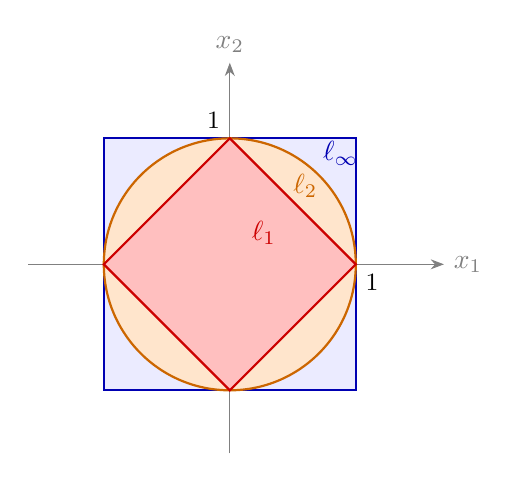
\begin{tikzpicture}[x=1.6cm, y=1.6cm, >=Stealth]
        \draw[->, gray] (-1.6,0) -- (1.7,0) node[right] {$x_1$};
        \draw[->, gray] (0,-1.5) -- (0,1.6) node[above] {$x_2$};
        \fill[blue!8] (-1,-1) -- (1,-1) -- (1,1) -- (-1,1) -- cycle;
        \fill[orange!20] (0,0) circle (1);
        \fill[red!25] (1,0) -- (0,1) -- (-1,0) -- (0,-1) -- cycle;
        \draw[blue!70!black, thick] (-1,-1) -- (1,-1) -- (1,1) -- (-1,1) -- cycle;
        \draw[orange!80!black, thick] (0,0) circle (1);
        \draw[red!80!black, thick] (1,0) -- (0,1) -- (-1,0) -- (0,-1) -- cycle;
        \node[red!80!black] at (0.27,0.25) {$\ell_1$};
        \node[orange!80!black] at (0.6,0.62) {$\ell_2$};
        \node[blue!70!black] at (0.88,0.88) {$\ell_\infty$};
        \node[below right] at (1,0) {\small $1$};
        \node[above left] at (0,1) {\small $1$};
    \end{tikzpicture}
    \caption[Unit balls of the $\ell_1$, $\ell_2$ and $\ell_\infty$ norms]{The unit balls $\{x \in \mathbb{R}^2 : \norm{x} \leq 1\}$ of the $\ell_1$ norm (red diamond), the $\ell_2$ norm (orange disk) and the $\ell_\infty$ norm (blue square). Each ball contains the previous one, in accordance with Proposition~\ref{prop:norm-comparison}.}
    \label{fig:unit-balls}
\end{figure}

\begin{proposition}\label{prop:norm-comparison}
    For every $x \in \mathbb{R}^n$,
    \[\norm{x}_\infty \leq \norm{x}_2 \leq \norm{x}_1 \leq n \norm{x}_\infty.\]
\end{proposition}

\begin{proof}
    Let $|x_k| = \norm{x}_\infty$ be the largest absolute value of an entry of $x$. Then $\norm{x}_\infty^2 = x_k^2 \leq x_1^2 + \cdots + x_n^2 = \norm{x}_2^2$. Next,
    \[\norm{x}_1^2 = \Big(\sum_i |x_i|\Big)^2 = \sum_i x_i^2 + \sum_{i \neq j} |x_i| |x_j| \geq \sum_i x_i^2 = \norm{x}_2^2.\]
    Finally, $\norm{x}_1 = \sum_i |x_i| \leq \sum_i |x_k| = n \norm{x}_\infty$.
\end{proof}

So all three norms are ``comparable'': if a vector is small in one of them, it is also small in the others (up to a factor that depends on $n$). In Example~\ref{ex:l1-l2} we improve the last inequality.

\begin{example}[Frobenius norm]
    In Lecture~1, we saw that the space $\mathbb{R}^{m \times n}$ of $m \times n$ matrices is a vector space, and it is isomorphic to $\mathbb{R}^{mn}$ by listing the entries of a matrix. The Euclidean norm of this list of entries is the Frobenius norm
    \[\norm{A}_F = \sqrt{\sum_{i=1}^m \sum_{j=1}^n A_{ij}^2} = \sqrt{\tr(A^\top A)},\]
    which is a norm on $\mathbb{R}^{m \times n}$.
\end{example}

\begin{remark}[Norms in machine learning]
    Norms are used to measure the size of model parameters. In regularized linear regression, we minimize the error of a model plus a penalty $\lambda \norm{w}$ on its weight vector $w$. With the squared $\ell_2$ norm (ridge regression), all weights are shrunk towards $0$. With the $\ell_1$ norm (the lasso), many weights become exactly $0$, which gives sparse models; one reason is that the $\ell_1$ unit ball in Figure~\ref{fig:unit-balls} has corners on the coordinate axes. The $\ell_\infty$ norm appears, for example, when we bound how much an adversary may change each pixel of an image.
\end{remark}

\section{Inner Products}

Norms measure lengths. To also measure angles, we need more structure: an inner product. The prototype is the dot product $x^\top y$ on $\mathbb{R}^n$.

\begin{definition}[Inner product]\label{def:inner-product}
    Let $V$ be a vector space. A function $\ip{\cdot}{\cdot}: V \times V \to \mathbb{R}$ is called
    \begin{itemize}
        \item bilinear if it is linear in each argument: for all $x, y, z \in V$ and $\lambda, \mu \in \mathbb{R}$,
        \[\ip{\lambda x + \mu y}{z} = \lambda \ip{x}{z} + \mu \ip{y}{z} \qquad \text{and} \qquad \ip{z}{\lambda x + \mu y} = \lambda \ip{z}{x} + \mu \ip{z}{y};\]
        \item symmetric if $\ip{x}{y} = \ip{y}{x}$ for all $x, y \in V$;
        \item positive definite if $\ip{x}{x} > 0$ for all $x \in V$ with $x \neq 0$.
    \end{itemize}
    An inner product on $V$ is a positive definite, symmetric, bilinear function $V \times V \to \mathbb{R}$. A vector space together with an inner product is called an inner product space.
\end{definition}

Note that $\ip{0}{x} = \ip{0 \cdot 0}{x} = 0 \cdot \ip{0}{x} = 0$ by bilinearity, so in particular $\ip{0}{0} = 0$.

\begin{example}[Dot product]\label{ex:dot}
    The dot product $\ip{x}{y} = x^\top y = \sum_i x_i y_i$ is an inner product on $\mathbb{R}^n$. It is bilinear and symmetric by the rules of matrix multiplication, and $x^\top x = x_1^2 + \cdots + x_n^2 > 0$ for $x \neq 0$. The space $\mathbb{R}^n$ with the dot product is called the Euclidean space. Unless we say otherwise, we always use the dot product on $\mathbb{R}^n$.
\end{example}

\begin{example}\label{ex:ip-A}
    On $\mathbb{R}^2$, define
    \[\ip{x}{y} = x_1 y_1 - (x_1 y_2 + x_2 y_1) + 2 x_2 y_2.\]
    This function is bilinear and symmetric. It is also positive definite, since
    \[\ip{x}{x} = x_1^2 - 2 x_1 x_2 + 2 x_2^2 = (x_1 - x_2)^2 + x_2^2 \geq 0,\]
    with equality only if $x_2 = 0$ and $x_1 = x_2$, i.e., $x = 0$. So it is an inner product, different from the dot product: for example, for $x = (1, 1)^\top$, we get $\ip{x}{x} = 1$, while $x^\top x = 2$.
\end{example}

\begin{example}
    \begin{itemize}
        \item For positive weights $w_1, \ldots, w_n > 0$, the weighted dot product $\ip{x}{y} = w_1 x_1 y_1 + \cdots + w_n x_n y_n$ is an inner product on $\mathbb{R}^n$. In machine learning, such weights can be used to make some features more important than others.
        \item The function $\ip{x}{y} = x_1 y_1 - x_2 y_2$ on $\mathbb{R}^2$ is bilinear and symmetric, but it is not an inner product, since $\ip{e_2}{e_2} = -1 < 0$.
        \item On the space $\mathbb{R}^{m \times n}$ of matrices, $\ip{A}{B} = \tr(A^\top B) = \sum_{i, j} A_{ij} B_{ij}$ is an inner product, the Frobenius inner product. It is the dot product of the lists of entries of $A$ and $B$.
    \end{itemize}
\end{example}

\subsection{Symmetric positive definite matrices}

All the inner products on $\mathbb{R}^n$ in the examples above can be written using a matrix. For instance, the inner product of Example~\ref{ex:ip-A} is
\[\ip{x}{y} = \begin{pmatrix} x_1 & x_2 \end{pmatrix} \begin{pmatrix} 1 & -1 \\ -1 & 2 \end{pmatrix} \begin{pmatrix} y_1 \\ y_2 \end{pmatrix} = x^\top A y.\]
The matrices that give inner products in this way are the following.

\begin{definition}[Symmetric positive definite matrix]\label{def:spd}
    A symmetric $n \times n$ matrix $A$ is called positive definite if
    \[x^\top A x > 0 \qquad \text{for all } x \in \mathbb{R}^n \text{ with } x \neq 0,\]
    and positive semidefinite if $x^\top A x \geq 0$ for all $x \in \mathbb{R}^n$. A symmetric positive definite matrix is also called an SPD matrix.
\end{definition}

\begin{theorem}\label{thm:spd}
    \begin{enumerate}
        \item If $A$ is a symmetric positive definite $n \times n$ matrix, then $\ip{x}{y}_A = x^\top A y$ is an inner product on $\mathbb{R}^n$.
        \item Conversely, let $\ip{\cdot}{\cdot}$ be an inner product on an $n$-dimensional vector space $V$, and let $\mathcal{B} = (b_1, \ldots, b_n)$ be an ordered basis of $V$. Let $A$ be the $n \times n$ matrix with entries $A_{ij} = \ip{b_i}{b_j}$. Then $A$ is symmetric positive definite, and
        \[\ip{x}{y} = [x]_{\mathcal{B}}^\top \, A \, [y]_{\mathcal{B}} \qquad \text{for all } x, y \in V,\]
        where $[x]_{\mathcal{B}}$ is the coordinate vector of $x$ with respect to $\mathcal{B}$, as in Lecture~1.
    \end{enumerate}
\end{theorem}

\begin{proof}
    (1) The function $x^\top A y$ is bilinear by the distributivity of matrix multiplication and the rules for scalars. It is symmetric, since $y^\top A x$ is a $1 \times 1$ matrix and therefore equal to its transpose $(y^\top A x)^\top = x^\top A^\top y = x^\top A y$. It is positive definite by assumption.

    (2) Write $x = \sum_i \psi_i b_i$ and $y = \sum_j \lambda_j b_j$, so that $[x]_{\mathcal{B}} = (\psi_1, \ldots, \psi_n)^\top$ and $[y]_{\mathcal{B}} = (\lambda_1, \ldots, \lambda_n)^\top$. By bilinearity,
    \[\ip{x}{y} = \Big\langle \sum_i \psi_i b_i, \sum_j \lambda_j b_j \Big\rangle = \sum_{i, j} \psi_i \ip{b_i}{b_j} \lambda_j = [x]_{\mathcal{B}}^\top A [y]_{\mathcal{B}}.\]
    The matrix $A$ is symmetric, since $\ip{b_i}{b_j} = \ip{b_j}{b_i}$. If $\psi \in \mathbb{R}^n$ is nonzero, then $x = \sum_i \psi_i b_i \neq 0$, since the $b_i$ are linearly independent, and hence $\psi^\top A \psi = \ip{x}{x} > 0$.
\end{proof}

The matrix $A$ in part 2 is called the Gram matrix of the basis $\mathcal{B}$. So, once we fix a basis, inner products on an $n$-dimensional space are the same thing as symmetric positive definite $n \times n$ matrices. The dot product on $\mathbb{R}^n$ corresponds to $A = I_n$ and the standard basis.

\begin{proposition}\label{prop:spd-properties}
    Let $A$ be a symmetric positive definite $n \times n$ matrix.
    \begin{enumerate}
        \item The diagonal entries of $A$ are positive.
        \item $A$ is invertible.
        \item For $n = 2$: a symmetric matrix $A = \begin{pmatrix} a & b \\ b & c \end{pmatrix}$ is positive definite if and only if $a > 0$ and $\det(A) = ac - b^2 > 0$.
    \end{enumerate}
\end{proposition}

\begin{proof}
    (1) $A_{ii} = e_i^\top A e_i > 0$.

    (2) If $Ax = 0$, then $x^\top A x = 0$, so $x = 0$. Hence $\Null(A) = \{0\}$, and $A$ is invertible by Lecture~1.

    (3) If $A$ is positive definite, then $a > 0$ by part 1. If $a > 0$, completing the square gives
    \[x^\top A x = a x_1^2 + 2b x_1 x_2 + c x_2^2 = a \Big(x_1 + \frac{b}{a} x_2\Big)^2 + \frac{ac - b^2}{a} x_2^2.\]
    If $ac - b^2 > 0$, both terms are nonnegative, and they are both zero only if $x_2 = 0$ and $x_1 = 0$; so $A$ is positive definite. If $ac - b^2 \leq 0$, then $x = (-b, a)^\top \neq 0$ gives $x^\top A x = (ac - b^2) a \leq 0$, so $A$ is not positive definite.
\end{proof}

For larger matrices, there is a similar test, Sylvester's criterion: a symmetric matrix is positive definite if and only if the determinants of all its upper left $k \times k$ submatrices, for $k = 1, \ldots, n$, are positive. We state it without proof. In Section~\ref{sec:spectral}, we will see another test, using eigenvalues (Corollary~\ref{cor:spd-eigenvalues}).

\begin{example}
    The matrix $A_1 = \begin{pmatrix} 9 & 6 \\ 6 & 5 \end{pmatrix}$ is positive definite, since $9 > 0$ and $\det(A_1) = 45 - 36 = 9 > 0$. Indeed, $x^\top A_1 x = (3x_1 + 2x_2)^2 + x_2^2$. The matrix $A_2 = \begin{pmatrix} 9 & 6 \\ 6 & 3 \end{pmatrix}$ is not, since $\det(A_2) = 27 - 36 = -9 < 0$: for $x = (2, -3)^\top$, we get $x^\top A_2 x = -9$.
\end{example}

\begin{example}\label{ex:BTB}
    Let $B$ be an $m \times n$ matrix with linearly independent columns. Then $B^\top B$ is symmetric positive definite: it is symmetric (Lecture~1), and for $x \neq 0$ we have $Bx \neq 0$, so
    \[x^\top B^\top B x = (Bx)^\top (Bx) = \norm{Bx}_2^2 > 0.\]
    Matrices of the form $B^\top B$ appear everywhere in machine learning, for example in linear regression (Section~\ref{sec:least-squares}) and as (scaled) covariance matrices of data.
\end{example}

\begin{remark}[Kernels]
    Many machine learning methods, such as support vector machines, only use the data through inner products $\ip{x_i}{x_j}$ of data points. Kernel methods replace them by $k(x_i, x_j) = \ip{\phi(x_i)}{\phi(x_j)}$, the inner product of the data after a (possibly nonlinear) feature map $\phi$. The matrix $K$ with entries $K_{ij} = k(x_i, x_j)$ is then a Gram matrix, and it is symmetric positive semidefinite.
\end{remark}

\section{Lengths and Distances}\label{sec:lengths}

\subsection{The norm of an inner product}

Every inner product gives a norm, in the same way that the dot product gives the Euclidean norm $\norm{x}_2 = \sqrt{x^\top x}$.

\begin{definition}[Induced norm]
    Let $V$ be an inner product space. The length, or norm, of a vector $x \in V$ is
    \[\norm{x} = \sqrt{\ip{x}{x}}.\]
    A vector $x$ with $\norm{x} = 1$ is called a unit vector. For $x \neq 0$, the vector $\frac{x}{\norm{x}}$ is a unit vector; replacing $x$ by $\frac{x}{\norm{x}}$ is called normalizing $x$.
\end{definition}

\begin{example}
    For $x = (1, 1)^\top$, the dot product gives $\norm{x} = \sqrt{2}$, while the inner product of Example~\ref{ex:ip-A} gives $\norm{x} = \sqrt{1} = 1$. So the length of a vector depends on the choice of the inner product.
\end{example}

To show that $\norm{x} = \sqrt{\ip{x}{x}}$ really is a norm, we need the most important inequality of linear algebra.

\begin{theorem}[Cauchy--Schwarz inequality]\label{thm:cauchy-schwarz}
    Let $V$ be an inner product space. For all $x, y \in V$,
    \[|\ip{x}{y}| \leq \norm{x} \, \norm{y},\]
    with equality if and only if $x$ and $y$ are linearly dependent.
\end{theorem}

\begin{proof}
    If $y = 0$, both sides are $0$, and $x$, $y$ are linearly dependent. So let $y \neq 0$. For every $t \in \mathbb{R}$, by bilinearity and symmetry,
    \[0 \leq \ip{x - ty}{x - ty} = \norm{x}^2 - 2t \ip{x}{y} + t^2 \norm{y}^2.\]
    Choosing $t = \frac{\ip{x}{y}}{\norm{y}^2}$ gives
    \[0 \leq \norm{x}^2 - 2\frac{\ip{x}{y}^2}{\norm{y}^2} + \frac{\ip{x}{y}^2}{\norm{y}^2} = \norm{x}^2 - \frac{\ip{x}{y}^2}{\norm{y}^2},\]
    i.e., $\ip{x}{y}^2 \leq \norm{x}^2 \norm{y}^2$. Taking square roots proves the inequality. Equality holds if and only if $\ip{x - ty}{x - ty} = 0$ for this $t$, i.e., $x = ty$, which (for $y \neq 0$) means that $x$ and $y$ are linearly dependent.
\end{proof}

\begin{corollary}\label{cor:induced-norm}
    If $V$ is an inner product space, then $\norm{x} = \sqrt{\ip{x}{x}}$ is a norm on $V$. In particular, the Euclidean norm $\norm{\cdot}_2$ is a norm on $\mathbb{R}^n$.
\end{corollary}

\begin{proof}
    Positive definiteness follows from the positive definiteness of the inner product, and $\norm{\lambda x} = \sqrt{\lambda^2 \ip{x}{x}} = |\lambda| \norm{x}$. For the triangle inequality, by the Cauchy--Schwarz inequality,
    \[\norm{x + y}^2 = \norm{x}^2 + 2 \ip{x}{y} + \norm{y}^2 \leq \norm{x}^2 + 2 \norm{x} \norm{y} + \norm{y}^2 = \big(\norm{x} + \norm{y}\big)^2. \qedhere\]
\end{proof}

\begin{example}\label{ex:l1-l2}
    Let $a = (|x_1|, \ldots, |x_n|)^\top$ and $\mathbf{1} = (1, \ldots, 1)^\top$. Applying the Cauchy--Schwarz inequality for the dot product to $a$ and $\mathbf{1}$ gives
    \[\norm{x}_1 = \sum_{i=1}^n |x_i| \cdot 1 \leq \sqrt{\sum_{i=1}^n x_i^2} \, \sqrt{\sum_{i=1}^n 1^2} = \sqrt{n} \, \norm{x}_2.\]
    This improves the inequality $\norm{x}_1 \leq n \norm{x}_\infty$ of Proposition~\ref{prop:norm-comparison}, since $\sqrt{n} \norm{x}_2 \leq n \norm{x}_\infty$.
\end{example}

Not every norm comes from an inner product. Norms that do come from an inner product can be recognized by the following identities.

\begin{proposition}[Parallelogram law and polarization]\label{prop:parallelogram}
    Let $V$ be an inner product space with the induced norm. For all $x, y \in V$:
    \begin{enumerate}
        \item $\norm{x + y}^2 + \norm{x - y}^2 = 2\norm{x}^2 + 2\norm{y}^2$ (parallelogram law);
        \item $\ip{x}{y} = \frac{1}{4}\big(\norm{x + y}^2 - \norm{x - y}^2\big)$ (polarization identity).
    \end{enumerate}
\end{proposition}

\begin{proof}
    Expanding with bilinearity, $\norm{x \pm y}^2 = \norm{x}^2 \pm 2\ip{x}{y} + \norm{y}^2$. Adding the two identities gives part 1; subtracting them gives part 2.
\end{proof}

The parallelogram law says that in a parallelogram, the sum of the squares of the two diagonals equals the sum of the squares of the four sides. The polarization identity shows that the inner product can be recovered from its norm.

\begin{example}
    The $\ell_1$ norm on $\mathbb{R}^2$ does not come from any inner product: for $x = e_1$ and $y = e_2$, we get $\norm{x + y}_1^2 + \norm{x - y}_1^2 = 4 + 4 = 8$, but $2\norm{x}_1^2 + 2\norm{y}_1^2 = 4$, so the parallelogram law fails. Hence normed spaces are more general than inner product spaces.
\end{example}

\subsection{Distances}

\begin{definition}[Distance]
    Let $V$ be an inner product space (or, more generally, a normed space). The distance between $x, y \in V$ is
    \[d(x, y) = \norm{x - y}.\]
    For the dot product on $\mathbb{R}^n$, this is the Euclidean distance $d(x, y) = \norm{x - y}_2 = \sqrt{\sum_i (x_i - y_i)^2}$.
\end{definition}

\begin{proposition}\label{prop:metric}
    The distance $d$ has the following properties, for all $x, y, z \in V$:
    \begin{enumerate}
        \item Positive definiteness: $d(x, y) \geq 0$, and $d(x, y) = 0$ if and only if $x = y$;
        \item Symmetry: $d(x, y) = d(y, x)$;
        \item Triangle inequality: $d(x, z) \leq d(x, y) + d(y, z)$.
    \end{enumerate}
\end{proposition}

\begin{proof}
    Part 1 follows from the positive definiteness of the norm, and part 2 from $\norm{x - y} = \norm{(-1)(y - x)} = \norm{y - x}$. Part 3 is the triangle inequality for the norm, applied to $x - z = (x - y) + (y - z)$.
\end{proof}

A function $d: X \times X \to \mathbb{R}$ on any set $X$ with these three properties is called a metric, and $(X, d)$ is called a metric space. So every normed space is a metric space.

\begin{example}
    For $x = (1, 2)^\top$ and $y = (4, 6)^\top$, we have $x - y = (-3, -4)^\top$, so the distance between $x$ and $y$ is
    \[\norm{x - y}_2 = \sqrt{9 + 16} = 5, \qquad \norm{x - y}_1 = 3 + 4 = 7, \qquad \norm{x - y}_\infty = 4\]
    for the Euclidean, Manhattan and maximum norms, respectively.
\end{example}

\begin{remark}[Distances in machine learning]
    The $k$-nearest neighbor method classifies a new data point by a majority vote among the $k$ training points that are closest to it. Which points are closest depends on the metric, so the choice of the norm matters. It also depends on the units of the features: if one feature is measured in meters and another in millimeters, the second one dominates the Euclidean distance. This is why features are usually standardized first, or, equivalently, a weighted inner product is used.
\end{remark}

\section{Angles and Orthogonality}

\subsection{Angles}

By the Cauchy--Schwarz inequality, $-1 \leq \frac{\ip{x}{y}}{\norm{x} \norm{y}} \leq 1$ for nonzero vectors $x$ and $y$. So the following definition makes sense.

\begin{definition}[Angle]
    Let $V$ be an inner product space, and let $x, y \in V$ be nonzero. The angle between $x$ and $y$ is the unique number $\omega \in [0, \pi]$ with
    \[\cos \omega = \frac{\ip{x}{y}}{\norm{x} \, \norm{y}}.\]
\end{definition}

For the dot product in $\mathbb{R}^2$ or $\mathbb{R}^3$, this is the usual angle between two arrows. Indeed, expanding $\norm{x - y}^2$ gives
\[\norm{x - y}^2 = \norm{x}^2 + \norm{y}^2 - 2 \ip{x}{y} = \norm{x}^2 + \norm{y}^2 - 2 \norm{x} \norm{y} \cos\omega,\]
which is the law of cosines for the triangle with sides $x$, $y$ and $x - y$ (see Figure~\ref{fig:angle}).

\begin{example}\label{ex:angle}
    The angle $\omega$ between $x = (3, 1)^\top$ and $y = (1, 2)^\top$ satisfies
    \[\cos\omega = \frac{3 \cdot 1 + 1 \cdot 2}{\sqrt{10} \, \sqrt{5}} = \frac{5}{\sqrt{50}} = \frac{1}{\sqrt{2}},\]
    so $\omega = \frac{\pi}{4}$, i.e., $45^\circ$.
\end{example}

\begin{figure}[ht]
    \centering
    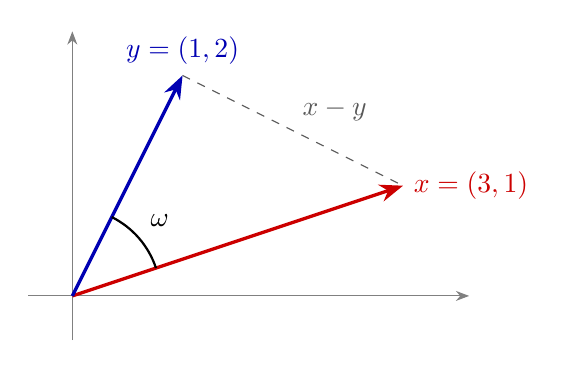
\begin{tikzpicture}[x=1.4cm, y=1.4cm, >=Stealth]
        \draw[->, gray] (-0.4,0) -- (3.6,0);
        \draw[->, gray] (0,-0.4) -- (0,2.4);
        \draw[->, very thick, red!80!black] (0,0) -- (3,1) node[right] {$x = (3, 1)$};
        \draw[->, very thick, blue!70!black] (0,0) -- (1,2) node[above] {$y = (1, 2)$};
        \draw[dashed, gray!70!black] (1,2) -- node[above right] {$x - y$} (3,1);
        \draw[thick] (18.43:0.8) arc[start angle=18.43, end angle=63.43, radius=0.8];
        \node at (40.93:1.05) {$\omega$};
    \end{tikzpicture}
    \caption[The angle between two vectors]{The angle $\omega = 45^\circ$ between $x = (3, 1)$ and $y = (1, 2)$ (Example~\ref{ex:angle}). The triangle with sides $x$, $y$ and $x - y$ satisfies the law of cosines.}
    \label{fig:angle}
\end{figure}

\subsection{Orthogonality}

\begin{definition}[Orthogonality]
    Two vectors $x$ and $y$ of an inner product space are orthogonal, written $x \perp y$, if $\ip{x}{y} = 0$. If, in addition, $\norm{x} = \norm{y} = 1$, then $x$ and $y$ are called orthonormal.
\end{definition}

So two nonzero vectors are orthogonal if and only if the angle between them is $\frac{\pi}{2}$. The zero vector is orthogonal to every vector.

\begin{example}\label{ex:orth-depends}
    The vectors $x = (1, 1)^\top$ and $y = (-1, 1)^\top$ are orthogonal for the dot product, since $x^\top y = -1 + 1 = 0$. Now consider the inner product $\ip{x}{y} = x^\top A y$ with $A = \diag(2, 1)$. Then
    \[\ip{x}{y} = 2 \cdot 1 \cdot (-1) + 1 \cdot 1 = -1, \qquad \norm{x}^2 = 2 + 1 = 3, \qquad \norm{y}^2 = 2 + 1 = 3,\]
    so $\cos\omega = -\frac{1}{3}$ and $\omega \approx 1.91 \approx 109.5^\circ$. So whether two vectors are orthogonal depends on the inner product.
\end{example}

\begin{theorem}[Pythagoras]\label{thm:pythagoras}
    If $x \perp y$, then $\norm{x + y}^2 = \norm{x}^2 + \norm{y}^2$.
\end{theorem}

\begin{proof}
    $\norm{x + y}^2 = \norm{x}^2 + 2\ip{x}{y} + \norm{y}^2 = \norm{x}^2 + \norm{y}^2$.
\end{proof}

\begin{remark}[Cosine similarity]
    In machine learning, the number $\cos\omega = \frac{\ip{x}{y}}{\norm{x} \norm{y}}$ is called the cosine similarity of $x$ and $y$. It is $1$ if $x$ and $y$ point in the same direction, $0$ if they are orthogonal, and $-1$ if they point in opposite directions. Unlike the distance, it does not change when $x$ or $y$ is multiplied by a positive scalar. This makes it useful for comparing text documents (represented by word counts, where long and short documents should be comparable) and embeddings, e.g., the vectors that language models assign to words and sentences.
\end{remark}

\subsection{Orthogonal matrices}

In Lecture~1, we defined an $n \times n$ matrix $Q$ to be orthogonal if $Q^\top Q = I_n$, and we claimed, without proof, that orthogonal matrices preserve lengths and angles. We can now make this precise.

\begin{theorem}\label{thm:orthogonal}
    For an $n \times n$ matrix $Q$, the following statements are equivalent:
    \begin{enumerate}
        \item $Q$ is orthogonal, i.e., $Q^\top Q = I_n$;
        \item $Q$ preserves the dot product: $(Qx)^\top (Qy) = x^\top y$ for all $x, y \in \mathbb{R}^n$;
        \item $Q$ preserves lengths: $\norm{Qx}_2 = \norm{x}_2$ for all $x \in \mathbb{R}^n$;
        \item the columns of $Q$ are orthonormal.
    \end{enumerate}
    In particular, orthogonal matrices preserve lengths, distances and angles.
\end{theorem}

\begin{proof}
    ($1 \Rightarrow 2$) $(Qx)^\top (Qy) = x^\top Q^\top Q y = x^\top y$.

    ($2 \Rightarrow 3$) Take $y = x$ and take square roots.

    ($3 \Rightarrow 2$) By the polarization identity (Proposition~\ref{prop:parallelogram}) and linearity,
    \[(Qx)^\top (Qy) = \tfrac{1}{4}\big(\norm{Qx + Qy}^2 - \norm{Qx - Qy}^2\big) = \tfrac{1}{4}\big(\norm{x + y}^2 - \norm{x - y}^2\big) = x^\top y.\]

    ($2 \Rightarrow 1$) The $(i, j)$ entry of $Q^\top Q$ is $e_i^\top Q^\top Q e_j = (Qe_i)^\top (Qe_j) = e_i^\top e_j$, which is $1$ if $i = j$ and $0$ otherwise.

    ($1 \Leftrightarrow 4$) The $(i, j)$ entry of $Q^\top Q$ is $q_i^\top q_j$, where $q_1, \ldots, q_n$ are the columns of $Q$. So $Q^\top Q = I_n$ means exactly that $q_i^\top q_j$ is $1$ for $i = j$ and $0$ for $i \neq j$.

    Finally, distances are lengths of differences, $\norm{Qx - Qy}_2 = \norm{Q(x - y)}_2 = \norm{x - y}_2$, and angles are defined in terms of the dot product and lengths.
\end{proof}

A map that preserves distances is called an isometry. Rotations and reflections are the typical examples; we study rotations in Section~\ref{sec:rotations}.

\section{Orthonormal Bases}

In $\mathbb{R}^n$, the standard basis $e_1, \ldots, e_n$ consists of vectors of length $1$ that are pairwise orthogonal. Bases with this property are especially convenient.

\begin{definition}[Orthonormal basis]
    Let $V$ be an inner product space. Vectors $b_1, \ldots, b_k \in V$ are called orthogonal if $\ip{b_i}{b_j} = 0$ for all $i \neq j$, and orthonormal if, in addition, $\norm{b_i} = 1$ for all $i$. In other words, $b_1, \ldots, b_k$ are orthonormal if
    \[\ip{b_i}{b_j} = \begin{cases} 1 & \text{if } i = j, \\ 0 & \text{if } i \neq j. \end{cases}\]
    An orthonormal basis (ONB) of $V$ is a basis of $V$ consisting of orthonormal vectors.
\end{definition}

\begin{lemma}\label{lem:orth-indep}
    Orthogonal nonzero vectors $b_1, \ldots, b_k$ are linearly independent.
\end{lemma}

\begin{proof}
    Suppose that $a_1 b_1 + \cdots + a_k b_k = 0$. Taking the inner product with $b_j$ and using bilinearity gives
    \[0 = \ip{a_1 b_1 + \cdots + a_k b_k}{b_j} = a_1 \ip{b_1}{b_j} + \cdots + a_k \ip{b_k}{b_j} = a_j \norm{b_j}^2.\]
    Since $b_j \neq 0$, we get $a_j = 0$, for every $j$.
\end{proof}

The main advantage of an orthonormal basis is that coordinates are computed by inner products, without solving a system of linear equations.

\begin{proposition}\label{prop:onb-coordinates}
    Let $b_1, \ldots, b_n$ be an orthonormal basis of $V$. Then for all $u, v \in V$:
    \begin{enumerate}
        \item $v = \ip{v}{b_1} b_1 + \ip{v}{b_2} b_2 + \cdots + \ip{v}{b_n} b_n$;
        \item $\ip{u}{v} = \sum_{i=1}^n \ip{u}{b_i} \ip{v}{b_i}$, and in particular $\norm{v}^2 = \sum_{i=1}^n \ip{v}{b_i}^2$ (Parseval's identity).
    \end{enumerate}
\end{proposition}

\begin{proof}
    (1) Write $v = c_1 b_1 + \cdots + c_n b_n$. Taking the inner product with $b_j$ gives $\ip{v}{b_j} = \sum_i c_i \ip{b_i}{b_j} = c_j$.

    (2) Write $u = \sum_i d_i b_i$ and $v = \sum_j c_j b_j$ with $d_i = \ip{u}{b_i}$ and $c_j = \ip{v}{b_j}$. Then $\ip{u}{v} = \sum_{i, j} d_i c_j \ip{b_i}{b_j} = \sum_i d_i c_i$.
\end{proof}

In the language of Theorem~\ref{thm:spd}: the Gram matrix of an orthonormal basis is the identity matrix, so in coordinates with respect to an orthonormal basis, every inner product becomes the dot product.

\begin{example}\label{ex:onb-r2}
    The vectors $b_1 = \frac{1}{\sqrt{2}}(1, 1)^\top$ and $b_2 = \frac{1}{\sqrt{2}}(1, -1)^\top$ form an orthonormal basis of $\mathbb{R}^2$. For $v = (3, 1)^\top$, we get
    \[\ip{v}{b_1} = \frac{4}{\sqrt{2}} = 2\sqrt{2}, \qquad \ip{v}{b_2} = \frac{2}{\sqrt{2}} = \sqrt{2},\]
    so $v = 2\sqrt{2}\, b_1 + \sqrt{2}\, b_2 = 2(1, 1)^\top + (1, -1)^\top$. Parseval's identity checks out: $(2\sqrt{2})^2 + (\sqrt{2})^2 = 10 = 3^2 + 1^2$.
\end{example}

\begin{remark}
    If $b_1, \ldots, b_n$ is an orthonormal basis of $\mathbb{R}^n$ (with the dot product), then the matrix $Q$ with columns $b_1, \ldots, b_n$ is orthogonal (Theorem~\ref{thm:orthogonal}). The coordinate vector of $v$ is then $Q^{-1} v = Q^\top v = (b_1^\top v, \ldots, b_n^\top v)^\top$, in agreement with Proposition~\ref{prop:onb-coordinates}.
\end{remark}

\subsection{The Gram--Schmidt process}

Every basis can be turned into an orthonormal basis. The idea is to go through the basis vectors one by one, and to subtract from each vector its components in the directions of the previous ones.

\begin{theorem}[Gram--Schmidt process]\label{thm:gram-schmidt}
    Let $v_1, \ldots, v_k$ be linearly independent vectors in an inner product space $V$. Define recursively, for $j = 1, \ldots, k$,
    \[u_j = v_j - \sum_{i=1}^{j-1} \ip{v_j}{e_i}\, e_i, \qquad e_j = \frac{u_j}{\norm{u_j}}.\]
    Then $e_1, \ldots, e_k$ are orthonormal, and $\Span\{e_1, \ldots, e_j\} = \Span\{v_1, \ldots, v_j\}$ for every $j = 1, \ldots, k$.
\end{theorem}

\begin{proof}
    We use induction on $j$. For $j = 1$, we have $u_1 = v_1 \neq 0$ and $e_1 = v_1 / \norm{v_1}$, so the claim holds. Now let $j \geq 2$, and assume that $e_1, \ldots, e_{j-1}$ are orthonormal with $\Span\{e_1, \ldots, e_{j-1}\} = \Span\{v_1, \ldots, v_{j-1}\}$.

    First, $u_j \neq 0$: otherwise $v_j = \sum_{i < j} \ip{v_j}{e_i} e_i$ would lie in $\Span\{e_1, \ldots, e_{j-1}\}$, which equals $\Span\{v_1, \ldots, v_{j-1}\}$, contradicting the linear independence of $v_1, \ldots, v_j$. So $e_j$ is well defined and has length $1$.

    Next, for $l < j$, using that $e_1, \ldots, e_{j-1}$ are orthonormal,
    \[\ip{u_j}{e_l} = \ip{v_j}{e_l} - \sum_{i < j} \ip{v_j}{e_i} \ip{e_i}{e_l} = \ip{v_j}{e_l} - \ip{v_j}{e_l} = 0,\]
    so $e_j$ is orthogonal to $e_1, \ldots, e_{j-1}$. Finally, $e_j$ is a linear combination of $v_j$ and $e_1, \ldots, e_{j-1}$, and conversely $v_j = \norm{u_j} e_j + \sum_{i < j} \ip{v_j}{e_i} e_i$. Together with the induction hypothesis, this gives $\Span\{e_1, \ldots, e_j\} = \Span\{v_1, \ldots, v_j\}$.
\end{proof}

The vector $\ip{v_j}{e_i} e_i$ is the component of $v_j$ in the direction of $e_i$; in Section~\ref{sec:projections}, we will call it the orthogonal projection of $v_j$ onto $\Span\{e_i\}$. In hand computations, it is often easier to postpone the normalization: since $\ip{v_j}{e_i} e_i = \frac{\ip{v_j}{u_i}}{\ip{u_i}{u_i}} u_i$, the vectors
\[u_j = v_j - \sum_{i=1}^{j-1} \frac{\ip{v_j}{u_i}}{\ip{u_i}{u_i}}\, u_i\]
are orthogonal, and we normalize them at the end. Figure~\ref{fig:gram-schmidt} illustrates the process for two vectors.

\begin{figure}[ht]
    \centering
    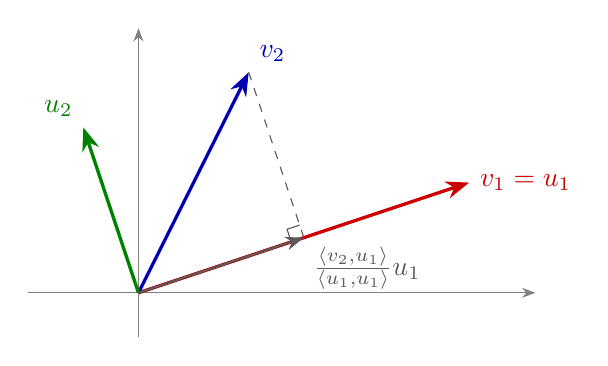
\begin{tikzpicture}[x=1.4cm, y=1.4cm, >=Stealth]
        \draw[->, gray] (-1,0) -- (3.6,0);
        \draw[->, gray] (0,-0.4) -- (0,2.4);
        \draw[->, very thick, red!80!black] (0,0) -- (3,1) node[right] {$v_1 = u_1$};
        \draw[->, very thick, blue!70!black] (0,0) -- (1,2) node[above right] {$v_2$};
        \draw[->, thick, gray!70!black] (0,0) -- (1.5,0.5);
        \node[below right, gray!70!black] at (1.5,0.5) {$\frac{\langle v_2, u_1 \rangle}{\langle u_1, u_1 \rangle} u_1$};
        \draw[dashed, gray!70!black] (1.5,0.5) -- (1,2);
        \draw[->, very thick, green!50!black] (0,0) -- (-0.5,1.5) node[above left] {$u_2$};
        \draw[gray!70!black] (1.386,0.462) -- (1.348,0.576) -- (1.462,0.614);
    \end{tikzpicture}
    \caption[The Gram--Schmidt process]{The Gram--Schmidt process for $v_1 = (3, 1)$ and $v_2 = (1, 2)$. The component of $v_2$ in the direction of $u_1 = v_1$ is $\frac{5}{10} u_1 = (1.5, 0.5)$; subtracting it gives $u_2 = (-0.5, 1.5)$, which is orthogonal to $u_1$. Normalizing $u_1$ and $u_2$ gives an orthonormal basis of $\mathbb{R}^2$.}
    \label{fig:gram-schmidt}
\end{figure}

\begin{example}\label{ex:gram-schmidt}
    Let us apply the Gram--Schmidt process to the basis $v_1 = (1, 1, 0)^\top$, $v_2 = (1, 0, 1)^\top$, $v_3 = (0, 1, 1)^\top$ of $\mathbb{R}^3$, using the unnormalized version:
    \begin{align*}
        u_1 &= v_1 = (1, 1, 0)^\top, \\
        u_2 &= v_2 - \frac{v_2^\top u_1}{u_1^\top u_1} u_1 = (1, 0, 1)^\top - \frac{1}{2}(1, 1, 0)^\top = \big(\tfrac{1}{2}, -\tfrac{1}{2}, 1\big)^\top, \\
        u_3 &= v_3 - \frac{v_3^\top u_1}{u_1^\top u_1} u_1 - \frac{v_3^\top u_2}{u_2^\top u_2} u_2 = (0, 1, 1)^\top - \frac{1}{2}(1, 1, 0)^\top - \frac{1/2}{3/2}\big(\tfrac{1}{2}, -\tfrac{1}{2}, 1\big)^\top = \big(-\tfrac{2}{3}, \tfrac{2}{3}, \tfrac{2}{3}\big)^\top.
    \end{align*}
    One checks that $u_1^\top u_2 = u_1^\top u_3 = u_2^\top u_3 = 0$. Normalizing gives the orthonormal basis
    \[e_1 = \frac{1}{\sqrt{2}} \begin{pmatrix} 1 \\ 1 \\ 0 \end{pmatrix}, \qquad e_2 = \frac{1}{\sqrt{6}} \begin{pmatrix} 1 \\ -1 \\ 2 \end{pmatrix}, \qquad e_3 = \frac{1}{\sqrt{3}} \begin{pmatrix} -1 \\ 1 \\ 1 \end{pmatrix}.\]
\end{example}

\begin{corollary}\label{cor:onb-exists}
    Every finite-dimensional inner product space has an orthonormal basis.
\end{corollary}

\begin{proof}
    Apply the Gram--Schmidt process to any basis $v_1, \ldots, v_n$. The resulting vectors $e_1, \ldots, e_n$ are orthonormal and span $\Span\{v_1, \ldots, v_n\} = V$, and they are linearly independent by Lemma~\ref{lem:orth-indep}.
\end{proof}

The Gram--Schmidt process can also be written as a factorization of matrices.

\begin{proposition}[QR decomposition]\label{prop:qr}
    Let $A$ be an $m \times n$ matrix with linearly independent columns $a_1, \ldots, a_n$. Then $A = QR$, where $Q$ is an $m \times n$ matrix with orthonormal columns (i.e., $Q^\top Q = I_n$), and $R$ is an upper triangular $n \times n$ matrix with positive diagonal entries.
\end{proposition}

\begin{proof}
    Apply the Gram--Schmidt process to $a_1, \ldots, a_n$ (with the dot product), and let $Q$ be the matrix with columns $e_1, \ldots, e_n$. Since $a_j \in \Span\{e_1, \ldots, e_j\}$ and $e_1, \ldots, e_j$ are orthonormal, the argument of Proposition~\ref{prop:onb-coordinates} gives $a_j = \sum_{i=1}^{j} (e_i^\top a_j)\, e_i$. So $A = QR$, where $R_{ij} = e_i^\top a_j$ for $i \leq j$ and $R_{ij} = 0$ for $i > j$. The diagonal entries are $R_{jj} = e_j^\top a_j = e_j^\top u_j = \norm{u_j} > 0$, since $a_j - u_j$ is a linear combination of $e_1, \ldots, e_{j-1}$, which are orthogonal to $e_j$.
\end{proof}

\begin{example}
    For the matrix $A$ with columns $v_1, v_2, v_3$ of Example~\ref{ex:gram-schmidt}, the matrix $Q$ has columns $e_1, e_2, e_3$, and
    \[R = Q^\top A = \begin{pmatrix} \sqrt{2} & \frac{1}{\sqrt{2}} & \frac{1}{\sqrt{2}} \\ 0 & \frac{\sqrt{6}}{2} & \frac{1}{\sqrt{6}} \\ 0 & 0 & \frac{2}{\sqrt{3}} \end{pmatrix}.\]
\end{example}

\begin{remark}
    In NumPy, \py{Q, R = np.linalg.qr(A)} computes a QR decomposition (the signs of some columns of $Q$ and rows of $R$ may differ from the ones above). It does not use the Gram--Schmidt process directly, since in floating-point arithmetic the vectors $e_j$ computed by the Gram--Schmidt process can be far from orthogonal; see Programming Exercise~P3. The QR decomposition is used, for example, to solve least squares problems in a numerically stable way.
\end{remark}

\section{Orthogonal Complements}

\begin{definition}[Orthogonal complement]
    Let $U$ be a subspace of an inner product space $V$. The orthogonal complement of $U$ is the set
    \[U^\perp = \{v \in V : \ip{v}{u} = 0 \text{ for all } u \in U\}\]
    of all vectors that are orthogonal to every vector of $U$.
\end{definition}

\begin{lemma}\label{lem:complement}
    Let $U$ be a subspace of an inner product space $V$.
    \begin{enumerate}
        \item $U^\perp$ is a subspace of $V$, and $U \cap U^\perp = \{0\}$.
        \item If $U = \Span\{u_1, \ldots, u_k\}$, then $v \in U^\perp$ if and only if $\ip{v}{u_i} = 0$ for $i = 1, \ldots, k$.
    \end{enumerate}
\end{lemma}

\begin{proof}
    (1) $\ip{0}{u} = 0$ for all $u$, so $0 \in U^\perp$. If $v, w \in U^\perp$ and $\lambda \in \mathbb{R}$, then $\ip{v + w}{u} = \ip{v}{u} + \ip{w}{u} = 0$ and $\ip{\lambda v}{u} = \lambda \ip{v}{u} = 0$ for all $u \in U$. If $v \in U \cap U^\perp$, then $\ip{v}{v} = 0$, so $v = 0$.

    (2) If $\ip{v}{u_i} = 0$ for all $i$, then $\ip{v}{\sum_i a_i u_i} = \sum_i a_i \ip{v}{u_i} = 0$ for every element $\sum_i a_i u_i$ of $U$. The converse is clear.
\end{proof}

To state the main theorem, we need the following notion.

\begin{definition}[Direct sum of subspaces]
    Let $U$ and $W$ be subspaces of a vector space $V$. We say that $V$ is the direct sum of $U$ and $W$, and write $V = U \oplus W$, if every $v \in V$ can be written in exactly one way as $v = u + w$ with $u \in U$ and $w \in W$.
\end{definition}

\begin{lemma}\label{lem:direct-sum-dim}
    If $V = U \oplus W$, where $U$ has a basis $u_1, \ldots, u_k$ and $W$ has a basis $w_1, \ldots, w_l$, then $u_1, \ldots, u_k, w_1, \ldots, w_l$ is a basis of $V$. In particular, $\dim V = \dim U + \dim W$.
\end{lemma}

\begin{proof}
    These vectors span $V$, since every $v = u + w$ is a linear combination of them. If $\sum_i a_i u_i + \sum_j b_j w_j = 0$, then $0 = \sum_i a_i u_i + \sum_j b_j w_j$ and $0 = 0 + 0$ are two ways to write $0$ as an element of $U$ plus an element of $W$. By uniqueness, $\sum_i a_i u_i = 0$ and $\sum_j b_j w_j = 0$, so all $a_i$ and $b_j$ are $0$.
\end{proof}

In the following theorem, we use the fact that every subspace of a finite-dimensional vector space is itself finite-dimensional; we state this without proof.

\begin{theorem}[Orthogonal decomposition]\label{thm:orth-decomposition}
    Let $U$ be a subspace of a finite-dimensional inner product space $V$. Then:
    \begin{enumerate}
        \item $V = U \oplus U^\perp$;
        \item $\dim U^\perp = \dim V - \dim U$;
        \item $(U^\perp)^\perp = U$.
    \end{enumerate}
\end{theorem}

\begin{proof}
    (1) By Corollary~\ref{cor:onb-exists}, $U$ has an orthonormal basis $e_1, \ldots, e_k$. For $v \in V$, let
    \[u = \sum_{i=1}^k \ip{v}{e_i} e_i \in U \qquad \text{and} \qquad w = v - u.\]
    Then $\ip{w}{e_j} = \ip{v}{e_j} - \ip{v}{e_j} = 0$ for all $j$, so $w \in U^\perp$ by Lemma~\ref{lem:complement}, and $v = u + w$. This decomposition is unique: if also $v = u' + w'$ with $u' \in U$ and $w' \in U^\perp$, then $u - u' = w' - w$ lies in $U \cap U^\perp = \{0\}$, so $u = u'$ and $w = w'$.

    (2) This follows from part 1 and Lemma~\ref{lem:direct-sum-dim}.

    (3) Every $u \in U$ is orthogonal to every vector of $U^\perp$, so $U \subseteq (U^\perp)^\perp$. Conversely, let $v \in (U^\perp)^\perp$, and write $v = u + w$ with $u \in U$ and $w \in U^\perp$. Then $0 = \ip{v}{w} = \ip{u}{w} + \ip{w}{w} = \norm{w}^2$, so $w = 0$ and $v = u \in U$.
\end{proof}

\begin{example}\label{ex:complement-line}
    Let $U = \Span\{(1, 1, 1)^\top\}$ in $\mathbb{R}^3$. By Lemma~\ref{lem:complement}, $U^\perp = \{x : x_1 + x_2 + x_3 = 0\}$ is the plane that we met as an example of a subspace in Lecture~1, and indeed $\dim U + \dim U^\perp = 1 + 2 = 3$. For $v = (1, 2, 3)^\top$, the proof of Theorem~\ref{thm:orth-decomposition} with $e_1 = \frac{1}{\sqrt{3}}(1, 1, 1)^\top$ gives the decomposition
    \[v = \underbrace{\frac{6}{\sqrt{3}} e_1}_{(2, 2, 2)^\top \in U} + \underbrace{(-1, 0, 1)^\top}_{\in U^\perp}.\]
\end{example}

\subsection{The four fundamental subspaces}

Orthogonal complements explain how the null space, the row space and the column space of a matrix from Lecture~1 fit together.

\begin{theorem}\label{thm:fundamental-subspaces}
    Let $A$ be an $m \times n$ matrix. Then, with respect to the dot product,
    \[\Null(A) = \row(A)^\perp \ \text{ in } \mathbb{R}^n \qquad \text{and} \qquad \Null(A^\top) = \col(A)^\perp \ \text{ in } \mathbb{R}^m.\]
\end{theorem}

\begin{proof}
    Let $r_1, \ldots, r_m$ be the rows of $A$, written as column vectors. The $i$-th entry of $Ax$ is $r_i^\top x$, so $Ax = 0$ if and only if $x$ is orthogonal to $r_1, \ldots, r_m$, which by Lemma~\ref{lem:complement} means $x \in \row(A)^\perp$. The second statement follows by applying the first one to $A^\top$, since $\row(A^\top) = \col(A)$.
\end{proof}

Combined with Theorem~\ref{thm:orth-decomposition}, this gives $\mathbb{R}^n = \row(A) \oplus \Null(A)$ and $\dim \row(A) + \dim \Null(A) = n$. Since $\dim \row(A) = \rank(A)$ (Lecture~1), this is another proof of the rank--nullity theorem.

\begin{example}
    In Lecture~1, we found that the null space of $A = \begin{pmatrix} 1 & 2 & -1 \\ 3 & -1 & 4 \end{pmatrix}$ is spanned by $(-1, 1, 1)^\top$. Indeed, this vector is orthogonal to both rows: $-1 + 2 - 1 = 0$ and $-3 - 1 + 4 = 0$.
\end{example}

\begin{remark}
    By Theorem~\ref{thm:orth-decomposition}(3), the second statement can also be written as $\col(A) = \Null(A^\top)^\perp$. So the system $Ax = b$ has a solution if and only if $b$ is orthogonal to every solution $y$ of $A^\top y = 0$.
\end{remark}

\subsection{Hyperplanes and linear classifiers}

\begin{definition}[Hyperplane]
    Let $w \in \mathbb{R}^n$ be nonzero and $c \in \mathbb{R}$. The set
    \[H = \{x \in \mathbb{R}^n : w^\top x = c\}\]
    is called a hyperplane, and $w$ is called a normal vector of $H$. If $c = 0$, then $H = \Span\{w\}^\perp$ is a subspace of dimension $n - 1$ (Theorem~\ref{thm:orth-decomposition}).
\end{definition}

If $c \neq 0$, the hyperplane $H$ does not contain $0$, so it is not a subspace. But if $x_0$ is any point of $H$, then $w^\top x = c$ if and only if $w^\top (x - x_0) = 0$. Hence
\[H = x_0 + \Span\{w\}^\perp = \{x_0 + u : u \in \Span\{w\}^\perp\}\]
is a shifted copy of the subspace $\Span\{w\}^\perp$. In general, a set of the form $x_0 + U$, where $U$ is a subspace, is called an affine subspace. In $\mathbb{R}^2$, hyperplanes are lines, and in $\mathbb{R}^3$, they are planes.

\begin{example}
    The plane $x + 2y + 2z = 2$ in $\mathbb{R}^3$ has the normal vector $w = (1, 2, 2)^\top$ and contains the point $x_0 = (2, 0, 0)^\top$. It is the shifted copy $x_0 + \Span\{w\}^\perp$ of the plane $x + 2y + 2z = 0$ through the origin.
\end{example}

\begin{remark}[Linear classifiers]\label{rem:linear-classifier}
    A linear classifier assigns to a data point $x \in \mathbb{R}^n$ the class
    \[f(x) = \sign(w^\top x + b) \in \{+1, -1\},\]
    for a weight vector $w$ and a bias $b \in \mathbb{R}$. The decision boundary $\{x : w^\top x + b = 0\}$ is a hyperplane with normal vector $w$, and the classifier predicts $+1$ on the side into which $w$ points (see Figure~\ref{fig:classifier}). The perceptron, logistic regression and support vector machines all learn classifiers of this form. In Section~\ref{sec:affine}, we compute the distance of a point to the decision boundary, which measures how confident the classification is.
\end{remark}

\begin{figure}[ht]
    \centering
    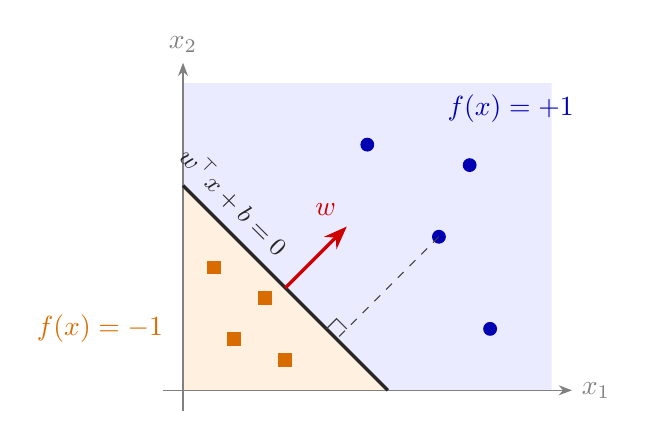
\begin{tikzpicture}[x=1.3cm, y=1.3cm, >=Stealth]
        \fill[blue!8] (2,0) -- (3.6,0) -- (3.6,3) -- (0,3) -- (0,2) -- cycle;
        \fill[orange!12] (0,0) -- (2,0) -- (0,2) -- cycle;
        \draw[->, gray] (-0.2,0) -- (3.8,0) node[right] {$x_1$};
        \draw[->, gray] (0,-0.2) -- (0,3.2) node[above] {$x_2$};
        \draw[very thick, gray!30!black] (0,2) -- (2,0);
        \node[gray!30!black, rotate=-45] at (0.5,1.85) {\small $w^\top x + b = 0$};
        \draw[->, very thick, red!80!black] (1,1) -- (1.6,1.6) node[above left] {$w$};
        \foreach \p in {(2.5,1.5), (3,0.6), (1.8,2.4), (2.8,2.2)} {
            \fill[blue!70!black] \p circle (2.5pt);
        }
        \foreach \p in {(0.5,0.5), (1,0.3), (0.3,1.2), (0.8,0.9)} {
            \fill[orange!85!black] \p ++(-2.5pt,-2.5pt) rectangle ++(5pt,5pt);
        }
        \draw[dashed, gray!50!black] (2.5,1.5) -- (1.5,0.5);
        \draw[gray!50!black] (1.6,0.6) -- (1.5,0.7) -- (1.4,0.6);
        \node[blue!70!black] at (3.2,2.75) {$f(x) = +1$};
        \node[orange!85!black, left] at (-0.1,0.6) {$f(x) = -1$};
    \end{tikzpicture}
    \caption[A linear classifier]{A linear classifier in $\mathbb{R}^2$ with $w = (1, 1)$ and $b = -2$. The decision boundary is the line $x_1 + x_2 = 2$ with normal vector $w$. Points on the side into which $w$ points (blue disks) are classified as $+1$, the others (orange squares) as $-1$. The dashed segment shows the distance of the point $(2.5, 1.5)$ to the boundary, which is $\sqrt{2}$ (Example~\ref{ex:classifier-distance}).}
    \label{fig:classifier}
\end{figure}

\section{Inner Products of Functions}

Inner products are not limited to $\mathbb{R}^n$. Functions can be added and multiplied by scalars (Lecture~1), and an integral gives a natural inner product on them.

\begin{proposition}\label{prop:function-ip}
    Let $C[a, b]$ be the vector space of continuous functions $f: [a, b] \to \mathbb{R}$, with pointwise addition and scalar multiplication. Then
    \[\ip{f}{g} = \int_a^b f(x) g(x) \, dx\]
    is an inner product on $C[a, b]$.
\end{proposition}

\begin{proof}
    Bilinearity and symmetry follow from the linearity of the integral. For positive definiteness, $\ip{f}{f} = \int_a^b f(x)^2 \, dx \geq 0$. If $f \neq 0$, then $f(x_0) \neq 0$ for some $x_0$, and by continuity, $f(x)^2 \geq \frac{1}{2} f(x_0)^2$ on some interval of positive length around $x_0$; hence $\ip{f}{f} > 0$.
\end{proof}

The continuity assumption matters: a function that is $1$ at a single point and $0$ everywhere else is nonzero, but the integral of its square is $0$.

\begin{example}
    On $C[-\pi, \pi]$, the functions $\sin$ and $\cos$ are orthogonal, since $\sin(x)\cos(x)$ is an odd function and therefore
    \[\ip{\sin}{\cos} = \int_{-\pi}^{\pi} \sin(x) \cos(x) \, dx = 0.\]
    Moreover, $\norm{\sin}^2 = \int_{-\pi}^{\pi} \sin^2(x) \, dx = \pi$. More generally, the functions $1$, $\cos(x)$, $\sin(x)$, $\cos(2x)$, $\sin(2x)$, \ldots{} are pairwise orthogonal on $[-\pi, \pi]$. Writing a function in terms of them is the idea behind Fourier series, which decompose a signal into frequencies.
\end{example}

\begin{example}[Legendre polynomials]\label{ex:legendre}
    Let us apply the Gram--Schmidt process (unnormalized version) to the polynomials $1, x, x^2, x^3$ in $C[-1, 1]$. We need the integrals $\int_{-1}^1 x^k \, dx$, which are $0$ for odd $k$ and $\frac{2}{k + 1}$ for even $k$:
    \begin{align*}
        u_0 &= 1, \\
        u_1 &= x - \frac{\ip{x}{1}}{\ip{1}{1}} \cdot 1 = x, \\
        u_2 &= x^2 - \frac{\ip{x^2}{1}}{\ip{1}{1}} \cdot 1 - \frac{\ip{x^2}{x}}{\ip{x}{x}} \, x = x^2 - \frac{2/3}{2} = x^2 - \frac{1}{3}, \\
        u_3 &= x^3 - \frac{\ip{x^3}{1}}{\ip{1}{1}} - \frac{\ip{x^3}{x}}{\ip{x}{x}} \, x - \frac{\ip{x^3}{u_2}}{\ip{u_2}{u_2}} \, u_2 = x^3 - \frac{2/5}{2/3} \, x = x^3 - \frac{3}{5} x.
    \end{align*}
    These orthogonal polynomials, shown in Figure~\ref{fig:legendre}, are (up to scaling) the Legendre polynomials. They are used, for example, to approximate functions by polynomials (Exercise~\ref{ex2:best-poly}).
\end{example}

\begin{figure}[ht]
    \centering
    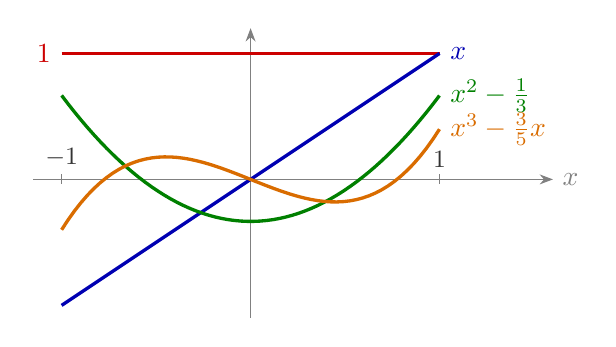
\begin{tikzpicture}[x=2.4cm, y=1.6cm, >=Stealth]
        \draw[->, gray] (-1.15,0) -- (1.6,0) node[right] {$x$};
        \draw[->, gray] (0,-1.1) -- (0,1.2);
        \foreach \t in {-1, 1} {
            \draw[gray] (\t,0.04) -- (\t,-0.04);
            \node[gray!40!black, above] at (\t,0.02) {\small $\t$};
        }
        \draw[very thick, red!80!black] (-1,1) node[left] {$1$} -- (1,1);
        \draw[very thick, blue!70!black] (-1,-1) -- (1,1) node[right] {$x$};
        \draw[very thick, green!50!black, domain=-1:1, samples=60] plot (\x, {\x*\x - 1/3}) node[right] {$x^2 - \frac{1}{3}$};
        \draw[very thick, orange!85!black, domain=-1:1, samples=60] plot (\x, {\x*\x*\x - 0.6*\x}) node[right] {$x^3 - \frac{3}{5}x$};
    \end{tikzpicture}
    \caption[Legendre polynomials]{The orthogonal polynomials of Example~\ref{ex:legendre} on $[-1, 1]$. Any two of them are orthogonal with respect to $\ip{f}{g} = \int_{-1}^1 f(x) g(x) \, dx$.}
    \label{fig:legendre}
\end{figure}

\begin{remark}[Random variables]
    Inner products also appear in probability. For random variables $X$ and $Y$ with mean $0$, the covariance $\mathrm{Cov}(X, Y) = \mathbb{E}[XY]$ behaves like an inner product: it is bilinear, symmetric, and $\mathrm{Cov}(X, X) = \mathrm{Var}(X) \geq 0$. The corresponding norm is the standard deviation, and the correlation coefficient $\frac{\mathrm{Cov}(X, Y)}{\sqrt{\mathrm{Var}(X)\mathrm{Var}(Y)}}$ is the cosine of the angle between $X$ and $Y$. In particular, uncorrelated random variables are orthogonal, and the Cauchy--Schwarz inequality shows that correlations lie between $-1$ and $1$.
\end{remark}

\section{Orthogonal Projections}\label{sec:projections}

Data in machine learning is often high-dimensional, and it is useful to replace each data point by a point of a lower-dimensional subspace while losing as little information as possible. The best way to do this, in a precise sense, is the orthogonal projection. Orthogonal projections are behind linear regression (Section~\ref{sec:least-squares}), principal component analysis (Section~\ref{sec:pca}) and the Gram--Schmidt process.

\begin{definition}[Orthogonal projection]
    Let $U$ be a subspace of a finite-dimensional inner product space $V$. By Theorem~\ref{thm:orth-decomposition}, every $v \in V$ can be written uniquely as $v = u + w$ with $u \in U$ and $w \in U^\perp$. The vector $\pi_U(v) = u$ is called the orthogonal projection of $v$ onto $U$. In other words, $\pi_U(v)$ is the unique vector with
    \[\pi_U(v) \in U \qquad \text{and} \qquad v - \pi_U(v) \in U^\perp.\]
\end{definition}

\begin{proposition}\label{prop:projection-properties}
    Let $U$ be a subspace of a finite-dimensional inner product space $V$.
    \begin{enumerate}
        \item If $e_1, \ldots, e_k$ is an orthonormal basis of $U$, then $\pi_U(v) = \sum_{i=1}^k \ip{v}{e_i} e_i$.
        \item $\pi_U: V \to V$ is a linear transformation with image $U$ and kernel $U^\perp$.
        \item $\pi_U \circ \pi_U = \pi_U$.
    \end{enumerate}
\end{proposition}

\begin{proof}
    (1) This is the formula from the proof of Theorem~\ref{thm:orth-decomposition}. (2) Linearity follows from the formula in part 1. The image is contained in $U$, and $\pi_U(u) = u$ for $u \in U$ (take $w = 0$), so the image is $U$. Moreover, $\pi_U(v) = 0$ if and only if $v = 0 + v$ with $v \in U^\perp$. (3) Since $\pi_U(v) \in U$, we get $\pi_U(\pi_U(v)) = \pi_U(v)$.
\end{proof}

A linear transformation $\pi$ with $\pi \circ \pi = \pi$ is called a projection; for matrices, this is the condition $P^2 = P$ (compare the idempotent matrices in the practice problems of Lecture~1).

\subsection{Projection onto a line}

\begin{proposition}\label{prop:projection-line}
    Let $b \neq 0$ and $U = \Span\{b\}$. Then
    \[\pi_U(x) = \frac{\ip{x}{b}}{\ip{b}{b}} \, b.\]
    For the dot product on $\mathbb{R}^n$, this is $\pi_U(x) = Px$ with the projection matrix
    \[P = \frac{b b^\top}{b^\top b},\]
    which is symmetric and satisfies $P^2 = P$.
\end{proposition}

\begin{proof}
    We look for $\pi_U(x) = \lambda b$ with $x - \lambda b \perp b$, i.e., $\ip{x}{b} - \lambda \ip{b}{b} = 0$. This gives $\lambda = \frac{\ip{x}{b}}{\ip{b}{b}}$. For the dot product, $\lambda b = b \lambda = \frac{b (b^\top x)}{b^\top b} = Px$. The matrix $b b^\top$ is symmetric, and $P^2 = \frac{b (b^\top b) b^\top}{(b^\top b)^2} = P$.
\end{proof}

Note that $bb^\top$ is an $n \times n$ matrix, while $b^\top b$ is a number. The length of the projection is $\norm{\pi_U(x)} = \frac{|\ip{x}{b}|}{\norm{b}} = \norm{x} \, |\cos\omega|$, where $\omega$ is the angle between $x$ and $b$, as in elementary geometry (Figure~\ref{fig:projection-line}).

\begin{figure}[ht]
    \centering
    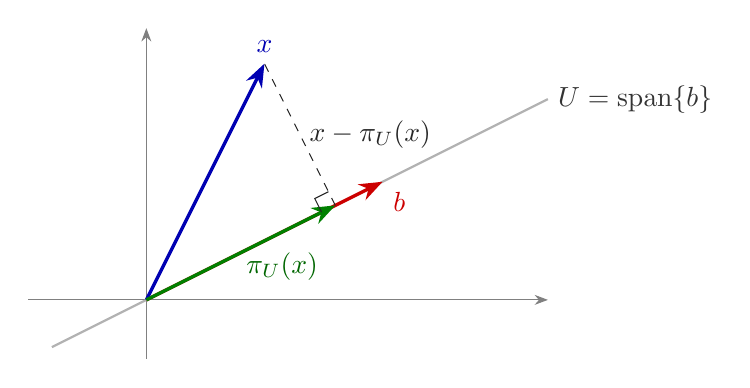
\begin{tikzpicture}[x=1.5cm, y=1.5cm, >=Stealth]
        \draw[->, gray] (-1,0) -- (3.4,0);
        \draw[->, gray] (0,-0.5) -- (0,2.3);
        \draw[thick, gray!60] (-0.8,-0.4) -- (3.4,1.7) node[right, gray!40!black] {$U = \Span\{b\}$};
        \draw[->, very thick, red!80!black] (0,0) -- (2,1) node[below right] {$b$};
        \draw[->, very thick, blue!70!black] (0,0) -- (1,2) node[above] {$x$};
        \draw[->, very thick, green!50!black] (0,0) -- (1.6,0.8);
        \node[green!40!black] at (1.15,0.28) {$\pi_U(x)$};
        \draw[dashed, gray!30!black] (1.6,0.8) -- node[right] {$x - \pi_U(x)$} (1,2);
        \draw[gray!30!black] (1.484,0.742) -- (1.426,0.858) -- (1.542,0.916);
    \end{tikzpicture}
    \caption[Projection onto a line]{The orthogonal projection of $x = (1, 2)$ onto the line spanned by $b = (2, 1)$ is $\pi_U(x) = \frac{4}{5} b = (1.6, 0.8)$. The difference $x - \pi_U(x) = (-0.6, 1.2)$ is orthogonal to $b$.}
    \label{fig:projection-line}
\end{figure}

\begin{example}
    Let $b = (1, 2, 2)^\top$ and $x = (1, 1, 1)^\top$. Then $b^\top b = 9$ and $b^\top x = 5$, so
    \[P = \frac{1}{9} \begin{pmatrix} 1 & 2 & 2 \\ 2 & 4 & 4 \\ 2 & 4 & 4 \end{pmatrix}, \qquad \pi_U(x) = Px = \frac{5}{9} \begin{pmatrix} 1 \\ 2 \\ 2 \end{pmatrix}.\]
    Indeed, $x - \pi_U(x) = \frac{1}{9}(4, -1, -1)^\top$ is orthogonal to $b$, since $4 - 2 - 2 = 0$.
\end{example}

\subsection{Projection onto a subspace}

Now let $U = \Span\{b_1, \ldots, b_m\}$ be an $m$-dimensional subspace of $\mathbb{R}^n$, with the dot product, and let $B$ be the $n \times m$ matrix with columns $b_1, \ldots, b_m$, so that $U = \col(B)$.

\begin{theorem}[Normal equations]\label{thm:projection-subspace}
    Let $B$ be an $n \times m$ matrix with linearly independent columns, and $U = \col(B)$. Then for every $x \in \mathbb{R}^n$,
    \[\pi_U(x) = B\lambda, \qquad \text{where } \lambda \in \mathbb{R}^m \text{ is the unique solution of } B^\top B \lambda = B^\top x.\]
    In other words, $\lambda = (B^\top B)^{-1} B^\top x$, and $\pi_U(x) = Px$ with the projection matrix
    \[P = B (B^\top B)^{-1} B^\top.\]
\end{theorem}

\begin{proof}
    Every vector of $U = \col(B)$ has the form $B\lambda$. By Theorem~\ref{thm:fundamental-subspaces}, $U^\perp = \col(B)^\perp = \Null(B^\top)$. So $B\lambda = \pi_U(x)$ if and only if $x - B\lambda \in \Null(B^\top)$, i.e., $B^\top(x - B\lambda) = 0$, i.e., $B^\top B \lambda = B^\top x$. The matrix $B^\top B$ is symmetric positive definite by Example~\ref{ex:BTB}, hence invertible by Proposition~\ref{prop:spd-properties}, so this equation has exactly one solution $\lambda = (B^\top B)^{-1} B^\top x$.
\end{proof}

The equations $B^\top B \lambda = B^\top x$ are called the normal equations, since they say that $x - B\lambda$ is orthogonal (``normal'') to $U$. If the columns of $B$ are orthonormal, then $B^\top B = I_m$, and the formulas simplify to $\lambda = B^\top x$ and $P = BB^\top$, in agreement with Proposition~\ref{prop:projection-properties}. For $m = 1$, we recover Proposition~\ref{prop:projection-line}.

\begin{example}\label{ex:projection-plane}
    Let $U = \Span\{(1, 1, 1)^\top, (0, 1, 2)^\top\}$ and $x = (6, 0, 0)^\top$. With $B = \begin{pmatrix} 1 & 0 \\ 1 & 1 \\ 1 & 2 \end{pmatrix}$, we get
    \[B^\top B = \begin{pmatrix} 3 & 3 \\ 3 & 5 \end{pmatrix}, \qquad B^\top x = \begin{pmatrix} 6 \\ 0 \end{pmatrix}, \qquad \lambda = \begin{pmatrix} 5 \\ -3 \end{pmatrix},\]
    where $\lambda$ solves the normal equations. Hence
    \[\pi_U(x) = 5 \begin{pmatrix} 1 \\ 1 \\ 1 \end{pmatrix} - 3 \begin{pmatrix} 0 \\ 1 \\ 2 \end{pmatrix} = \begin{pmatrix} 5 \\ 2 \\ -1 \end{pmatrix}, \qquad x - \pi_U(x) = \begin{pmatrix} 1 \\ -2 \\ 1 \end{pmatrix},\]
    and indeed $x - \pi_U(x)$ is orthogonal to both columns of $B$. The projection matrix is
    \[P = B (B^\top B)^{-1} B^\top = \frac{1}{6} \begin{pmatrix} 5 & 2 & -1 \\ 2 & 2 & 2 \\ -1 & 2 & 5 \end{pmatrix}.\]
\end{example}

\begin{proposition}\label{prop:projection-matrix}
    The projection matrix $P = B(B^\top B)^{-1}B^\top$ is symmetric, and $P^2 = P$.
\end{proposition}

\begin{proof}
    $P^2 = B(B^\top B)^{-1} (B^\top B) (B^\top B)^{-1} B^\top = B (B^\top B)^{-1} B^\top = P$. Since $B^\top B$ is symmetric, so is its inverse (Lecture~1: $(A^{-1})^\top = (A^\top)^{-1}$), and therefore $P^\top = B \big((B^\top B)^{-1}\big)^\top B^\top = P$.
\end{proof}

The most important property of the orthogonal projection is that it gives the closest point.

\begin{theorem}[Best approximation]\label{thm:best-approximation}
    Let $U$ be a subspace of a finite-dimensional inner product space $V$, and let $v \in V$. Then $\pi_U(v)$ is the point of $U$ that is closest to $v$:
    \[\norm{v - \pi_U(v)} < \norm{v - u} \qquad \text{for every } u \in U \text{ with } u \neq \pi_U(v).\]
\end{theorem}

\begin{proof}
    Write $v - u = \big(v - \pi_U(v)\big) + \big(\pi_U(v) - u\big)$. The first summand lies in $U^\perp$, and the second one in $U$, so they are orthogonal. By the theorem of Pythagoras,
    \[\norm{v - u}^2 = \norm{v - \pi_U(v)}^2 + \norm{\pi_U(v) - u}^2 > \norm{v - \pi_U(v)}^2,\]
    since $\pi_U(v) - u \neq 0$.
\end{proof}

The number $\norm{v - \pi_U(v)}$ is called the distance from $v$ to $U$. In Example~\ref{ex:projection-plane}, the distance from $x$ to the plane $U$ is $\norm{(1, -2, 1)^\top} = \sqrt{6}$.

\begin{remark}
    The Gram--Schmidt process (Theorem~\ref{thm:gram-schmidt}) can now be described in one line: $u_j = v_j - \pi_{U_{j-1}}(v_j)$, where $U_{j-1} = \Span\{v_1, \ldots, v_{j-1}\}$. That is, we subtract from $v_j$ its projection onto the span of the previous vectors.
\end{remark}

\subsection{Least squares and linear regression}\label{sec:least-squares}

Suppose we are given data points $(x_1, y_1), \ldots, (x_N, y_N)$ with $x_i, y_i \in \mathbb{R}$, and we want to find the line $y = w_0 + w_1 x$ that fits the data best. In general, no line passes through all points, so we look for the line that minimizes the sum of squared errors
\[\sum_{i=1}^N \big(y_i - (w_0 + w_1 x_i)\big)^2 = \norm{y - Aw}^2, \qquad \text{where} \quad A = \begin{pmatrix} 1 & x_1 \\ \vdots & \vdots \\ 1 & x_N \end{pmatrix}, \quad y = \begin{pmatrix} y_1 \\ \vdots \\ y_N \end{pmatrix}, \quad w = \begin{pmatrix} w_0 \\ w_1 \end{pmatrix}.\]
The matrix $A$ is called the design matrix. This is a special case of the following problem.

\begin{theorem}[Least squares]\label{thm:least-squares}
    Let $A$ be an $N \times n$ matrix with linearly independent columns, and let $y \in \mathbb{R}^N$. Then there is exactly one $w^* \in \mathbb{R}^n$ that minimizes $\norm{y - Aw}$, namely the solution of the normal equations
    \[A^\top A \, w^* = A^\top y, \qquad \text{i.e.,} \qquad w^* = (A^\top A)^{-1} A^\top y.\]
    Moreover, $Aw^* = \pi_{\col(A)}(y)$.
\end{theorem}

\begin{proof}
    As $w$ ranges over $\mathbb{R}^n$, the vector $Aw$ ranges over $\col(A)$. By Theorem~\ref{thm:best-approximation}, $\norm{y - Aw}$ is minimal exactly when $Aw = \pi_{\col(A)}(y)$, and by Theorem~\ref{thm:projection-subspace} (with $B = A$ and $\lambda = w$), this happens exactly for $w = (A^\top A)^{-1} A^\top y$.
\end{proof}

\begin{example}\label{ex:regression}
    Let us fit a line to the data points $(-1, 0)$, $(0, 1)$ and $(1, 3)$. The design matrix and the normal equations are
    \[A = \begin{pmatrix} 1 & -1 \\ 1 & 0 \\ 1 & 1 \end{pmatrix}, \quad y = \begin{pmatrix} 0 \\ 1 \\ 3 \end{pmatrix}, \qquad A^\top A = \begin{pmatrix} 3 & 0 \\ 0 & 2 \end{pmatrix}, \quad A^\top y = \begin{pmatrix} 4 \\ 3 \end{pmatrix},\]
    so $w^* = \big(\frac{4}{3}, \frac{3}{2}\big)^\top$, and the best line is $y = \frac{4}{3} + \frac{3}{2} x$ (Figure~\ref{fig:regression}). The fitted values are $Aw^* = \big(-\frac{1}{6}, \frac{4}{3}, \frac{17}{6}\big)^\top$, the residuals are $y - Aw^* = \big(\frac{1}{6}, -\frac{1}{3}, \frac{1}{6}\big)^\top$, and the minimal sum of squared errors is $\frac{1}{36} + \frac{1}{9} + \frac{1}{36} = \frac{1}{6}$. As predicted by the theory, the residual vector is orthogonal to both columns of $A$: its entries sum to $0$, and $-\frac{1}{6} + 0 + \frac{1}{6} = 0$.
\end{example}

\begin{figure}[ht]
    \centering
    \begin{tikzpicture}[x=1.5cm, y=1.5cm, >=Stealth]
        \draw[->, gray] (-1.8,0) -- (1.9,0) node[right] {$x$};
        \draw[->, gray] (0,-1) -- (0,3.9) node[above] {$y$};
        \draw[gray] (-1,0.06) -- (-1,-0.06);
        \node[gray!40!black, above left] at (-1,0) {\small $-1$};
        \draw[gray] (1,0.06) -- (1,-0.06) node[below] {\small $1$};
        \foreach \t in {1, 2, 3} {
            \draw[gray] (0.06,\t) -- (-0.06,\t) node[left] {\small $\t$};
        }
        \draw[very thick, blue!70!black, domain=-1.4:1.6] plot (\x, {4/3 + 1.5*\x}) node[right] {$y = \frac{4}{3} + \frac{3}{2}x$};
        \draw[ultra thick, red!80!black] (-1,0) -- (-1,-1/6);
        \draw[ultra thick, red!80!black] (0,1) -- (0,4/3);
        \draw[ultra thick, red!80!black] (1,3) -- (1,17/6);
        \foreach \p in {(-1,0), (0,1), (1,3)} {
            \fill[orange!85!black] \p circle (2pt);
        }
    \end{tikzpicture}
    \caption[Least squares regression]{The least squares line for the data points $(-1, 0)$, $(0, 1)$, $(1, 3)$ (Example~\ref{ex:regression}). The red segments are the residuals; the line minimizes the sum of their squared lengths.}
    \label{fig:regression}
\end{figure}

\begin{remark}[Linear regression in machine learning]
    The same method works for any number of features: each row of the design matrix $A$ contains the features of one data point (and a $1$ for the intercept $w_0$), and the least squares solution gives the weights of the linear model. Using the columns $1, x, x^2, \ldots, x^d$, we can also fit polynomials of degree $d$ (polynomial regression). In practice, the normal equations are not solved by computing $(A^\top A)^{-1}$, but with a QR decomposition or with \py{np.linalg.lstsq}, which are more accurate (compare Lecture~1).
\end{remark}

\subsection{Projections onto affine subspaces and distances to hyperplanes}\label{sec:affine}

Let $L = x_0 + U$ be an affine subspace, i.e., a subspace $U$ shifted by a vector $x_0$. To project onto $L$, we shift everything by $-x_0$, project onto $U$, and shift back:
\[\pi_L(x) = x_0 + \pi_U(x - x_0).\]
Then $x - \pi_L(x) = (x - x_0) - \pi_U(x - x_0)$ lies in $U^\perp$, and by Theorem~\ref{thm:best-approximation}, $\pi_L(x)$ is the point of $L$ closest to $x$.

\begin{theorem}[Distance to a hyperplane]\label{thm:distance-hyperplane}
    Let $H = \{z \in \mathbb{R}^n : w^\top z = c\}$ be a hyperplane, where $w \neq 0$. For every $x \in \mathbb{R}^n$, the point of $H$ closest to $x$ is
    \[\pi_H(x) = x - \frac{w^\top x - c}{\norm{w}^2}\, w, \qquad \text{and the distance from } x \text{ to } H \text{ is} \qquad \frac{|w^\top x - c|}{\norm{w}}.\]
\end{theorem}

\begin{proof}
    Let $x_0 \in H$, so that $H = x_0 + W$ with $W = \Span\{w\}^\perp$, and $W^\perp = \Span\{w\}$ by Theorem~\ref{thm:orth-decomposition}(3). Since $v = \pi_W(v) + \pi_{W^\perp}(v)$ for every $v$, we get
    \[x - \pi_H(x) = (x - x_0) - \pi_W(x - x_0) = \pi_{\Span\{w\}}(x - x_0) = \frac{w^\top (x - x_0)}{w^\top w}\, w = \frac{w^\top x - c}{\norm{w}^2}\, w,\]
    using Proposition~\ref{prop:projection-line} and $w^\top x_0 = c$. Taking the norm gives the distance.
\end{proof}

The number $\frac{w^\top x - c}{\norm{w}}$, without the absolute value, is called the signed distance: it is positive on the side of $H$ into which $w$ points, and negative on the other side.

\begin{example}
    The distance from the point $x = (1, 2, 3)^\top$ to the plane $H$ given by $x + 2y + 2z = 2$ is
    \[\frac{|1 + 4 + 6 - 2|}{\sqrt{1 + 4 + 4}} = \frac{9}{3} = 3,\]
    and the closest point of $H$ is $\pi_H(x) = (1, 2, 3)^\top - \frac{9}{9}(1, 2, 2)^\top = (0, 0, 1)^\top$.
\end{example}

\begin{example}\label{ex:classifier-distance}
    For the linear classifier of Figure~\ref{fig:classifier}, with $w = (1, 1)^\top$ and $b = -2$, the decision boundary is the hyperplane $w^\top x = 2$. The signed distance of the point $x = (2.5, 1.5)^\top$ to it is $\frac{w^\top x + b}{\norm{w}} = \frac{4 - 2}{\sqrt{2}} = \sqrt{2}$, and the closest point on the boundary is $(2.5, 1.5)^\top - \frac{2}{2}(1, 1)^\top = (1.5, 0.5)^\top$.
\end{example}

\begin{remark}[Margins]
    For a linear classifier, the distance of a data point to the decision boundary is a measure of confidence: points far from the boundary are classified with a large margin. Support vector machines choose the hyperplane that maximizes the smallest distance from the training points to the boundary, which by Theorem~\ref{thm:distance-hyperplane} means maximizing $\min_i \frac{|w^\top x_i + b|}{\norm{w}}$.
\end{remark}

\section{Rotations}\label{sec:rotations}

\begin{definition}[Rotation]
    A rotation of $\mathbb{R}^n$ is an orthogonal $n \times n$ matrix $R$ with $\det(R) = 1$. The set of rotations is denoted by $\mathrm{SO}(n)$, the special orthogonal group.
\end{definition}

By Theorem~\ref{thm:orthogonal}, rotations preserve lengths, distances and angles, and the condition $\det(R) = 1$ means that they preserve the orientation (Lecture~1). Orthogonal matrices with determinant $-1$, such as reflections, reverse the orientation. Since products and inverses of orthogonal matrices are orthogonal, and $\det(R_1 R_2) = \det(R_1)\det(R_2)$, products and inverses of rotations are again rotations; so $\mathrm{SO}(n)$ is a matrix group. The inverse of a rotation $R$ is simply $R^\top$.

\subsection{Rotations in the plane}

In Lecture~1, we met the rotation matrices
\[R_\theta = \begin{pmatrix} \cos\theta & -\sin\theta \\ \sin\theta & \cos\theta \end{pmatrix},\]
which rotate the plane counterclockwise by the angle $\theta$. One can show (see the practice problems of Lecture~1) that every rotation of $\mathbb{R}^2$ is of this form. Since $R_\alpha R_\beta = R_{\alpha + \beta} = R_\beta R_\alpha$, rotations of the plane commute with each other.

\subsection{Rotations in three dimensions}

The rotations of $\mathbb{R}^3$ by the angle $\theta$ about the three coordinate axes are
\[R_1(\theta) = \begin{pmatrix} 1 & 0 & 0 \\ 0 & \cos\theta & -\sin\theta \\ 0 & \sin\theta & \cos\theta \end{pmatrix}, \quad R_2(\theta) = \begin{pmatrix} \cos\theta & 0 & \sin\theta \\ 0 & 1 & 0 \\ -\sin\theta & 0 & \cos\theta \end{pmatrix}, \quad R_3(\theta) = \begin{pmatrix} \cos\theta & -\sin\theta & 0 \\ \sin\theta & \cos\theta & 0 \\ 0 & 0 & 1 \end{pmatrix}.\]
For example, $R_3(\theta)$ fixes the $x_3$-axis and rotates the $x_1 x_2$-plane by $\theta$. Each of them is orthogonal with determinant $1$. Every rotation of $\mathbb{R}^3$ can be written as a product of such rotations, and it fixes a line through the origin, its axis (we do not prove these facts here).

\begin{example}
    Unlike in the plane, rotations of $\mathbb{R}^3$ do not commute in general. For $\theta = \frac{\pi}{2}$,
    \[R_1\big(\tfrac{\pi}{2}\big) R_3\big(\tfrac{\pi}{2}\big) = \begin{pmatrix} 0 & -1 & 0 \\ 0 & 0 & -1 \\ 1 & 0 & 0 \end{pmatrix} \neq \begin{pmatrix} 0 & 0 & 1 \\ 1 & 0 & 0 \\ 0 & 1 & 0 \end{pmatrix} = R_3\big(\tfrac{\pi}{2}\big) R_1\big(\tfrac{\pi}{2}\big).\]
    For instance, the first product maps $e_1$ to $e_3$, while the second maps $e_1$ to $e_2$. You can check this with a book: rotate it first about one axis and then about another, and compare with the opposite order.
\end{example}

\subsection{\texorpdfstring{Rotations in $n$ dimensions}{Rotations in n dimensions}}

\begin{definition}[Givens rotation]
    For $1 \leq i < j \leq n$ and an angle $\theta$, the Givens rotation $G_{ij}(\theta)$ is the $n \times n$ matrix that agrees with the identity matrix, except for the four entries
    \[G_{ii} = \cos\theta, \qquad G_{ij} = -\sin\theta, \qquad G_{ji} = \sin\theta, \qquad G_{jj} = \cos\theta.\]
\end{definition}

The Givens rotation $G_{ij}(\theta)$ rotates the plane spanned by $e_i$ and $e_j$ by the angle $\theta$, and fixes all other standard basis vectors. Its columns are orthonormal, and its determinant is $\cos^2\theta + \sin^2\theta = 1$ (expand along the other rows), so it is a rotation. Givens rotations are used in numerical linear algebra: a well-chosen Givens rotation makes a chosen entry of a matrix zero, and a sequence of them computes a QR decomposition.

\begin{remark}[Rotations in machine learning]
    Since rotations preserve dot products and distances, any method that only depends on distances or dot products between data points, such as $k$-nearest neighbors with the Euclidean distance, gives the same results after the data is rotated. In contrast, methods such as decision trees, which look at individual coordinates, may change. Rotated copies of images are also used for data augmentation, to make image classifiers robust to rotations.
\end{remark}

\section{The Spectral Theorem}\label{sec:spectral}

In Lecture~1, we saw that a matrix is diagonalizable if it has a basis of eigenvectors, and that some matrices, such as the shear or a rotation, are not diagonalizable. Symmetric matrices are much better behaved: they always have an orthonormal basis of eigenvectors. Symmetric matrices are everywhere in machine learning: covariance matrices, Gram and kernel matrices, and the matrices $A^\top A$ of least squares problems are all symmetric.

To state the theorem, we use complex eigenvalues (Lecture~1). For a vector $v \in \mathbb{C}^n$, we write $\bar{v}$ for the vector of complex conjugates of its entries. Then $\bar{v}^\top v = \sum_i \bar{v}_i v_i = \sum_i |v_i|^2 > 0$ for $v \neq 0$. A complex number $\lambda$ is a root of $p_A$ if and only if $Av = \lambda v$ for some nonzero $v \in \mathbb{C}^n$, by the same argument as for real eigenvalues.

\begin{theorem}[Spectral theorem]\label{thm:spectral}
    Let $A$ be a symmetric real $n \times n$ matrix. Then:
    \begin{enumerate}
        \item all complex eigenvalues of $A$ are real;
        \item eigenvectors of $A$ for distinct eigenvalues are orthogonal;
        \item there is an orthonormal basis $q_1, \ldots, q_n$ of $\mathbb{R}^n$ consisting of eigenvectors of $A$. Equivalently,
        \[A = Q \Lambda Q^\top,\]
        where $Q$ is the orthogonal matrix with columns $q_1, \ldots, q_n$, and $\Lambda = \diag(\lambda_1, \ldots, \lambda_n)$ contains the corresponding eigenvalues.
    \end{enumerate}
\end{theorem}

\begin{proof}
    (1) Let $Av = \lambda v$ with $\lambda \in \mathbb{C}$ and $v \in \mathbb{C}^n$, $v \neq 0$. The number $z = \bar{v}^\top A v$ is real: since $A$ is real and symmetric, its complex conjugate is $\bar{z} = v^\top A \bar{v} = (v^\top A \bar{v})^\top = \bar{v}^\top A^\top v = z$. Since $z = \bar{v}^\top (\lambda v) = \lambda\, \bar{v}^\top v$, we get $\lambda = z / (\bar{v}^\top v) \in \mathbb{R}$.

    (2) Let $Av = \lambda v$ and $Aw = \mu w$ with $\lambda \neq \mu$. Then
    \[\lambda\, v^\top w = (Av)^\top w = v^\top A^\top w = v^\top A w = \mu\, v^\top w,\]
    so $(\lambda - \mu) v^\top w = 0$, and hence $v^\top w = 0$.

    (3) We use induction on $n$; the case $n = 1$ is clear. By part 1 and the fundamental theorem of algebra, $p_A$ has a real root $\lambda_1$. Let $q_1$ be a unit eigenvector for $\lambda_1$ (it can be chosen real, since $A - \lambda_1 I_n$ is a real matrix with a nonzero null space). Let $W = \Span\{q_1\}^\perp$, and let $w_2, \ldots, w_n$ be an orthonormal basis of $W$ (Theorem~\ref{thm:orth-decomposition} and Corollary~\ref{cor:onb-exists}). The subspace $W$ is mapped into itself by $A$: if $x \in W$, then $q_1^\top (Ax) = (Aq_1)^\top x = \lambda_1 q_1^\top x = 0$.

    Let $M$ be the $n \times (n-1)$ matrix with columns $w_2, \ldots, w_n$, so that $M^\top M = I_{n-1}$, and let $B = M^\top A M$, which is a symmetric $(n-1) \times (n-1)$ matrix. Since $Aw_i \in W$, Proposition~\ref{prop:onb-coordinates} gives $Aw_i = \sum_k (w_k^\top A w_i) w_k$, i.e., $AM = MB$. By induction, $B$ has an orthonormal basis of eigenvectors $y_2, \ldots, y_n \in \mathbb{R}^{n-1}$, with $By_j = \lambda_j y_j$. Then the vectors $q_j = M y_j$ ($j = 2, \ldots, n$) are orthonormal, since $q_i^\top q_j = y_i^\top M^\top M y_j = y_i^\top y_j$; they lie in $W$, so they are orthogonal to $q_1$; and they are eigenvectors, since $Aq_j = AMy_j = MBy_j = \lambda_j q_j$. So $q_1, \ldots, q_n$ is an orthonormal basis of eigenvectors.

    Finally, by Theorem~\ref{thm:orthogonal}, $Q$ is orthogonal, so $Q^{-1} = Q^\top$, and by the diagonalization theorem of Lecture~1, $A = Q\Lambda Q^{-1} = Q\Lambda Q^\top$.
\end{proof}

The factorization $A = Q\Lambda Q^\top$ is called the eigendecomposition, or spectral decomposition, of $A$. Multiplying out, it says that
\[A = \lambda_1 q_1 q_1^\top + \lambda_2 q_2 q_2^\top + \cdots + \lambda_n q_n q_n^\top,\]
where each $q_i q_i^\top$ is the matrix of the orthogonal projection onto the line $\Span\{q_i\}$ (Proposition~\ref{prop:projection-line}). So a symmetric matrix projects a vector onto $n$ orthogonal directions, scales the projections by the eigenvalues, and adds them up.

\begin{example}\label{ex:spectral}
    Let $A = \begin{pmatrix} 2 & 1 & 1 \\ 1 & 2 & 1 \\ 1 & 1 & 2 \end{pmatrix} = J + 2I_3$, where $J = \begin{pmatrix} 0 & 1 & 1 \\ 1 & 0 & 1 \\ 1 & 1 & 0 \end{pmatrix}$ is the matrix from the section on eigenvalues in Lecture~1. By the computations there, the eigenvalues of $A$ are $2 + 2 = 4$, with eigenspace $\Span\{(1, 1, 1)^\top\}$, and $-1 + 2 = 1$, with eigenspace the plane $x + y + z = 0$. As predicted by the spectral theorem, the two eigenspaces are orthogonal. To get an orthonormal basis of the plane, we apply the Gram--Schmidt process to its basis $(1, -1, 0)^\top$, $(1, 0, -1)^\top$, which gives $\frac{1}{\sqrt{2}}(1, -1, 0)^\top$ and $\frac{1}{\sqrt{6}}(1, 1, -2)^\top$. Hence $A = Q\Lambda Q^\top$ with
    \[Q = \begin{pmatrix} \frac{1}{\sqrt{3}} & \frac{1}{\sqrt{2}} & \frac{1}{\sqrt{6}} \\ \frac{1}{\sqrt{3}} & -\frac{1}{\sqrt{2}} & \frac{1}{\sqrt{6}} \\ \frac{1}{\sqrt{3}} & 0 & -\frac{2}{\sqrt{6}} \end{pmatrix}, \qquad \Lambda = \diag(4, 1, 1).\]
\end{example}

\begin{corollary}\label{cor:spd-eigenvalues}
    A symmetric matrix is positive definite if and only if all its eigenvalues are positive, and positive semidefinite if and only if all its eigenvalues are nonnegative.
\end{corollary}

\begin{proof}
    Write $A = Q\Lambda Q^\top$ and $y = Q^\top x$. Then
    \[x^\top A x = y^\top \Lambda y = \lambda_1 y_1^2 + \cdots + \lambda_n y_n^2.\]
    If all $\lambda_i > 0$, this is positive for $x \neq 0$ (then $y \neq 0$, since $Q^\top$ is invertible). Conversely, $q_i^\top A q_i = \lambda_i$, so if $A$ is positive definite, all $\lambda_i > 0$. The semidefinite case is the same, with $\geq$ instead of $>$.
\end{proof}

\begin{example}
    The matrix $\begin{pmatrix} 9 & 6 \\ 6 & 5 \end{pmatrix}$ from the subsection on symmetric positive definite matrices has trace $14$ and determinant $9$, so its eigenvalues $7 \pm 2\sqrt{10}$ are both positive, and it is positive definite. The matrix $\begin{pmatrix} 9 & 6 \\ 6 & 3 \end{pmatrix}$ has determinant $-9 < 0$, so its eigenvalues have opposite signs (their product is negative), and it is not positive definite.
\end{example}

\begin{proposition}[Rayleigh quotient]\label{prop:rayleigh}
    Let $A$ be symmetric with eigenvalues $\lambda_1 \geq \lambda_2 \geq \cdots \geq \lambda_n$ and orthonormal eigenvectors $q_1, \ldots, q_n$. Then for every $x \neq 0$,
    \[\lambda_n \leq \frac{x^\top A x}{x^\top x} \leq \lambda_1,\]
    with equality on the right for $x = q_1$, and on the left for $x = q_n$.
\end{proposition}

\begin{proof}
    With $y = Q^\top x$, we have $x^\top x = y^\top y$ (Theorem~\ref{thm:orthogonal}) and $x^\top A x = \sum_i \lambda_i y_i^2$, which lies between $\lambda_n \sum_i y_i^2$ and $\lambda_1 \sum_i y_i^2$. For $x = q_i$, the quotient is $q_i^\top A q_i = \lambda_i$.
\end{proof}

So the largest eigenvalue of a symmetric matrix is the maximum of $x^\top A x$ over all unit vectors $x$, and it is attained at an eigenvector. This is the key to principal component analysis.

\begin{remark}[Geometry of symmetric positive definite matrices]
    If $A$ is symmetric positive definite, the set $\{x : x^\top A x = 1\}$ is an ellipse (in $\mathbb{R}^2$) or an ellipsoid (in higher dimensions), whose axes point in the directions of the eigenvectors $q_i$ and have lengths $\frac{1}{\sqrt{\lambda_i}}$, since in the coordinates $y = Q^\top x$ the equation becomes $\lambda_1 y_1^2 + \cdots + \lambda_n y_n^2 = 1$. In machine learning, such ellipsoids describe the shape of Gaussian distributions (with $A$ the inverse covariance matrix) and the shape of the loss surface of least squares problems near a minimum; when the eigenvalues have very different sizes, gradient descent zig-zags and converges slowly.
\end{remark}

\section{The Singular Value Decomposition}\label{sec:svd}

The eigendecomposition only exists for square matrices, and in general only for diagonalizable ones. The singular value decomposition (SVD) exists for every matrix, square or not. It is one of the most useful factorizations in applied mathematics and machine learning: it describes the geometry of every linear transformation, gives the best low-rank approximations of a matrix, and is the basis of principal component analysis.

\subsection{Existence of the SVD}

\begin{theorem}[Singular value decomposition]\label{thm:svd}
    Let $A$ be a real $m \times n$ matrix. Then there are an orthogonal $m \times m$ matrix $U$, an orthogonal $n \times n$ matrix $V$, and an $m \times n$ matrix $\Sigma$ with
    \[\Sigma_{11} = \sigma_1 \geq \Sigma_{22} = \sigma_2 \geq \cdots \geq \Sigma_{rr} = \sigma_r > 0\]
    and all other entries $0$, such that
    \[A = U \Sigma V^\top.\]
    The number $r$ of nonzero diagonal entries is the rank of $A$. The numbers $\sigma_1, \ldots, \sigma_r$ are called the singular values of $A$; the columns $u_1, \ldots, u_m$ of $U$ and $v_1, \ldots, v_n$ of $V$ are called the left and right singular vectors of $A$.
\end{theorem}

\begin{proof}
    The $n \times n$ matrix $A^\top A$ is symmetric, and positive semidefinite, since $x^\top A^\top A x = \norm{Ax}^2 \geq 0$. By the spectral theorem and Corollary~\ref{cor:spd-eigenvalues}, there is an orthonormal basis $v_1, \ldots, v_n$ of $\mathbb{R}^n$ of eigenvectors of $A^\top A$, with eigenvalues $\lambda_1 \geq \cdots \geq \lambda_n \geq 0$ (we order them by size). Note that
    \[\norm{Av_i}^2 = v_i^\top A^\top A v_i = \lambda_i \, v_i^\top v_i = \lambda_i.\]
    Let $r$ be the number of positive eigenvalues, and let $\sigma_i = \sqrt{\lambda_i}$ and $u_i = \frac{1}{\sigma_i} A v_i$ for $i = 1, \ldots, r$. These vectors are orthonormal:
    \[u_i^\top u_j = \frac{v_i^\top A^\top A v_j}{\sigma_i \sigma_j} = \frac{\lambda_j\, v_i^\top v_j}{\sigma_i \sigma_j} = \begin{cases} 1 & \text{if } i = j, \\ 0 & \text{if } i \neq j. \end{cases}\]
    Let $u_{r+1}, \ldots, u_m$ be an orthonormal basis of $\Span\{u_1, \ldots, u_r\}^\perp$ (Theorem~\ref{thm:orth-decomposition} and Corollary~\ref{cor:onb-exists}), so that $u_1, \ldots, u_m$ is an orthonormal basis of $\mathbb{R}^m$, and let $U$ and $V$ be the orthogonal matrices with these columns. For $i \leq r$, we have $Av_i = \sigma_i u_i$ by definition, and for $i > r$, we have $\norm{Av_i}^2 = \lambda_i = 0$, so $Av_i = 0$. Column by column, this says that $AV = U\Sigma$, and hence $A = U\Sigma V^{-1} = U\Sigma V^\top$.

    Finally, every vector $Ax = \sum_i (v_i^\top x) Av_i = \sum_{i \leq r} \sigma_i (v_i^\top x) u_i$ lies in $\Span\{u_1, \ldots, u_r\}$, and conversely $u_i = A\big(\frac{1}{\sigma_i} v_i\big) \in \col(A)$. So $\col(A) = \Span\{u_1, \ldots, u_r\}$, and since $u_1, \ldots, u_r$ are linearly independent (Lemma~\ref{lem:orth-indep}), $\rank(A) = r$.
\end{proof}

The proof shows how to compute the SVD by hand:
\begin{enumerate}
    \item compute the eigenvalues $\lambda_1 \geq \cdots \geq \lambda_n$ and orthonormal eigenvectors $v_1, \ldots, v_n$ of $A^\top A$;
    \item set $\sigma_i = \sqrt{\lambda_i}$ and $u_i = \frac{1}{\sigma_i} A v_i$ for the positive eigenvalues;
    \item complete $u_1, \ldots, u_r$ to an orthonormal basis of $\mathbb{R}^m$.
\end{enumerate}
Similarly, $AA^\top = U \Sigma\Sigma^\top U^\top$, so the left singular vectors are eigenvectors of $AA^\top$, with the same nonzero eigenvalues $\sigma_i^2$.

\begin{example}\label{ex:svd-3x2}
    Let $A = \begin{pmatrix} 1 & 1 \\ 0 & 1 \\ 1 & 0 \end{pmatrix}$. Then $A^\top A = \begin{pmatrix} 2 & 1 \\ 1 & 2 \end{pmatrix}$, which we diagonalized in Lecture~1: its eigenvalues are $3$ and $1$, with orthonormal eigenvectors $v_1 = \frac{1}{\sqrt{2}}(1, 1)^\top$ and $v_2 = \frac{1}{\sqrt{2}}(1, -1)^\top$. So $\sigma_1 = \sqrt{3}$ and $\sigma_2 = 1$, and
    \[u_1 = \frac{1}{\sqrt{3}} A v_1 = \frac{1}{\sqrt{6}} \begin{pmatrix} 2 \\ 1 \\ 1 \end{pmatrix}, \qquad u_2 = \frac{1}{1} A v_2 = \frac{1}{\sqrt{2}} \begin{pmatrix} 0 \\ -1 \\ 1 \end{pmatrix}.\]
    A unit vector orthogonal to both is $u_3 = \frac{1}{\sqrt{3}}(1, -1, -1)^\top$. Hence
    \[\begin{pmatrix} 1 & 1 \\ 0 & 1 \\ 1 & 0 \end{pmatrix} = \underbrace{\begin{pmatrix} \frac{2}{\sqrt{6}} & 0 & \frac{1}{\sqrt{3}} \\ \frac{1}{\sqrt{6}} & -\frac{1}{\sqrt{2}} & -\frac{1}{\sqrt{3}} \\ \frac{1}{\sqrt{6}} & \frac{1}{\sqrt{2}} & -\frac{1}{\sqrt{3}} \end{pmatrix}}_{U} \underbrace{\begin{pmatrix} \sqrt{3} & 0 \\ 0 & 1 \\ 0 & 0 \end{pmatrix}}_{\Sigma} \underbrace{\frac{1}{\sqrt{2}}\begin{pmatrix} 1 & 1 \\ 1 & -1 \end{pmatrix}}_{V^\top}.\]
\end{example}

\subsection{The geometry of the SVD}

Since $U$ and $V$ are orthogonal, the SVD says that every linear transformation $x \mapsto Ax$ is a composition of three simple steps: an orthogonal transformation $V^\top$ (a rotation, possibly combined with a reflection), a scaling $\Sigma$ of the coordinate axes by the singular values (which may also change the dimension), and another orthogonal transformation $U$. In particular, $A$ maps the unit sphere of $\mathbb{R}^n$ to an ellipsoid (possibly flattened) in $\mathbb{R}^m$, whose semi-axes are $\sigma_1 u_1, \ldots, \sigma_r u_r$: the right singular vector $v_i$ is mapped to $\sigma_i u_i$.

\begin{example}[The SVD of a shear]\label{ex:svd-shear}
    Let $A = \begin{pmatrix} 1 & 1 \\ 0 & 1 \end{pmatrix}$ be the shear from the gallery of linear transformations in Lecture~1. Then $A^\top A = \begin{pmatrix} 1 & 1 \\ 1 & 2 \end{pmatrix}$ has trace $3$ and determinant $1$, so its eigenvalues are $\frac{3 \pm \sqrt{5}}{2} = \varphi^2$ and $\varphi^{-2}$, where $\varphi = \frac{1 + \sqrt{5}}{2}$ is the golden ratio, which we met in Lecture~1 in Binet's formula for the Fibonacci numbers. So the singular values of the shear are
    \[\sigma_1 = \varphi \approx 1.618 \qquad \text{and} \qquad \sigma_2 = \frac{1}{\varphi} \approx 0.618.\]
    Using $\varphi^2 = \varphi + 1$, one checks that, with $c = \sqrt{1 + \varphi^2}$,
    \[v_1 = \frac{1}{c}\begin{pmatrix} 1 \\ \varphi \end{pmatrix}, \quad v_2 = \frac{1}{c}\begin{pmatrix} -\varphi \\ 1 \end{pmatrix}, \quad u_1 = \frac{1}{c}\begin{pmatrix} \varphi \\ 1 \end{pmatrix}, \quad u_2 = \frac{1}{c}\begin{pmatrix} -1 \\ \varphi \end{pmatrix}.\]
    Both $U$ and $V$ are rotations, by the angles $31.7^\circ$ and $58.3^\circ$. So the shear is the same as: rotate by $-58.3^\circ$, stretch the $x$-axis by $\varphi$ and shrink the $y$-axis by $\frac{1}{\varphi}$, and rotate by $31.7^\circ$ (Figure~\ref{fig:svd}).
\end{example}

\begin{figure}[ht]
    \centering
    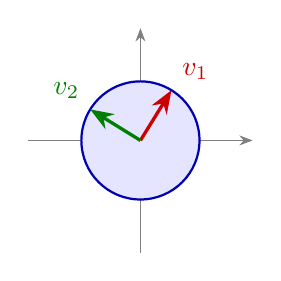
\begin{tikzpicture}[x=0.75cm, y=0.75cm, >=Stealth, baseline=(current bounding box.center)]
        \draw[->, gray] (-1.9,0) -- (1.9,0);
        \draw[->, gray] (0,-1.9) -- (0,1.9);
        \fill[blue!10] (0,0) circle (1);
        \draw[blue!70!black, thick] (0,0) circle (1);
        \draw[->, very thick, red!80!black] (0,0) -- (0.526,0.851) node[above right] {$v_1$};
        \draw[->, very thick, green!50!black] (0,0) -- (-0.851,0.526) node[above left] {$v_2$};
    \end{tikzpicture}
    $\xrightarrow{\ V^\top\ }$
    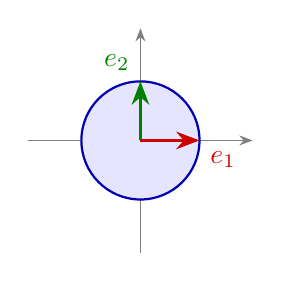
\begin{tikzpicture}[x=0.75cm, y=0.75cm, >=Stealth, baseline=(current bounding box.center)]
        \draw[->, gray] (-1.9,0) -- (1.9,0);
        \draw[->, gray] (0,-1.9) -- (0,1.9);
        \fill[blue!10] (0,0) circle (1);
        \draw[blue!70!black, thick] (0,0) circle (1);
        \draw[->, very thick, red!80!black] (0,0) -- (1,0) node[below right] {$e_1$};
        \draw[->, very thick, green!50!black] (0,0) -- (0,1) node[above left] {$e_2$};
    \end{tikzpicture}
    $\xrightarrow{\ \Sigma\ }$
    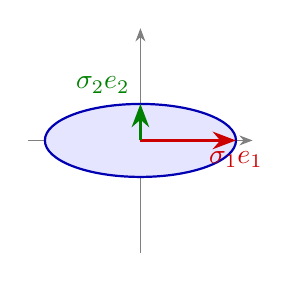
\begin{tikzpicture}[x=0.75cm, y=0.75cm, >=Stealth, baseline=(current bounding box.center)]
        \draw[->, gray] (-1.9,0) -- (1.9,0);
        \draw[->, gray] (0,-1.9) -- (0,1.9);
        \fill[blue!10] (0,0) ellipse [x radius=1.618, y radius=0.618];
        \draw[blue!70!black, thick] (0,0) ellipse [x radius=1.618, y radius=0.618];
        \draw[->, very thick, red!80!black] (0,0) -- (1.618,0) node[below] {$\sigma_1 e_1$};
        \draw[->, very thick, green!50!black] (0,0) -- (0,0.618) node[above left] {$\sigma_2 e_2$};
    \end{tikzpicture}
    $\xrightarrow{\ U\ }$
    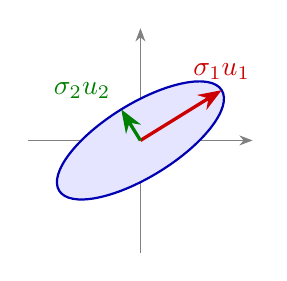
\begin{tikzpicture}[x=0.75cm, y=0.75cm, >=Stealth, baseline=(current bounding box.center)]
        \draw[->, gray] (-1.9,0) -- (1.9,0);
        \draw[->, gray] (0,-1.9) -- (0,1.9);
        \fill[blue!10, rotate=31.72] (0,0) ellipse [x radius=1.618, y radius=0.618];
        \draw[blue!70!black, thick, rotate=31.72] (0,0) ellipse [x radius=1.618, y radius=0.618];
        \draw[->, very thick, red!80!black] (0,0) -- (1.376,0.851) node[above] {$\sigma_1 u_1$};
        \draw[->, very thick, green!50!black] (0,0) -- (-0.325,0.526) node[above left] {$\sigma_2 u_2$};
    \end{tikzpicture}
    \caption[The geometry of the SVD]{The SVD of the shear $A = \begin{pmatrix} 1 & 1 \\ 0 & 1 \end{pmatrix}$ (Example~\ref{ex:svd-shear}). The rotation $V^\top$ moves the right singular vectors $v_1, v_2$ to $e_1, e_2$; the scaling $\Sigma$ stretches the axes by $\sigma_1 = \varphi$ and $\sigma_2 = 1/\varphi$; and the rotation $U$ moves the axes to the left singular vectors. Altogether, the unit circle is mapped to an ellipse with semi-axes $\sigma_1 u_1 = Av_1$ and $\sigma_2 u_2 = Av_2$.}
    \label{fig:svd}
\end{figure}

\begin{proposition}\label{prop:svd-subspaces}
    Let $A = U\Sigma V^\top$ be an SVD of a matrix $A$ of rank $r$. Then
    \[A = \sigma_1 u_1 v_1^\top + \sigma_2 u_2 v_2^\top + \cdots + \sigma_r u_r v_r^\top,\]
    and the four fundamental subspaces of $A$ are
    \begin{align*}
        \col(A) &= \Span\{u_1, \ldots, u_r\}, & \Null(A^\top) &= \Span\{u_{r+1}, \ldots, u_m\}, \\
        \row(A) &= \Span\{v_1, \ldots, v_r\}, & \Null(A) &= \Span\{v_{r+1}, \ldots, v_n\}.
    \end{align*}
\end{proposition}

\begin{proof}
    For every $x$, we saw in the proof of Theorem~\ref{thm:svd} that $Ax = \sum_{i \leq r} \sigma_i u_i (v_i^\top x)$, which is the first formula applied to $x$. The formula for $\col(A)$ was also shown there. If $x = \sum_i c_i v_i$, then $Ax = \sum_{i \leq r} \sigma_i c_i u_i$, which is $0$ if and only if $c_1 = \cdots = c_r = 0$; this gives $\Null(A)$. In an orthonormal basis, the orthogonal complement of the span of some basis vectors is the span of the other ones, so the remaining two formulas follow from Theorem~\ref{thm:fundamental-subspaces} and Theorem~\ref{thm:orth-decomposition}(3).
\end{proof}

The first formula writes $A$ as a sum of $r$ matrices of rank $1$. It also gives the reduced SVD $A = U_r \Sigma_r V_r^\top$, where $U_r$ and $V_r$ consist of the first $r$ columns of $U$ and $V$, and $\Sigma_r = \diag(\sigma_1, \ldots, \sigma_r)$; NumPy computes it with \py{np.linalg.svd(A, full_matrices=False)}.

\subsection{Matrix norms and low-rank approximation}

\begin{definition}[Spectral norm]
    The spectral norm (or operator norm) of an $m \times n$ matrix $A$ is
    \[\norm{A}_2 = \max_{x \neq 0} \frac{\norm{Ax}}{\norm{x}},\]
    the largest factor by which $A$ stretches a vector.
\end{definition}

\begin{proposition}\label{prop:matrix-norms}
    Let $A$ have singular values $\sigma_1 \geq \cdots \geq \sigma_r > 0$. Then
    \[\norm{A}_2 = \sigma_1 \qquad \text{and} \qquad \norm{A}_F = \sqrt{\sigma_1^2 + \cdots + \sigma_r^2}.\]
\end{proposition}

\begin{proof}
    $\frac{\norm{Ax}^2}{\norm{x}^2} = \frac{x^\top A^\top A x}{x^\top x}$ is the Rayleigh quotient of $A^\top A$, whose largest eigenvalue is $\sigma_1^2$; so the maximum is $\sigma_1$ by Proposition~\ref{prop:rayleigh}. For the Frobenius norm, $\norm{A}_F^2 = \tr(A^\top A)$ is the sum of the eigenvalues of $A^\top A$ (by Lecture~1, the trace is the sum of the eigenvalues), which is $\sigma_1^2 + \cdots + \sigma_r^2$.
\end{proof}

The rank-$1$ expansion suggests approximating $A$ by keeping only the terms with the largest singular values. This is the best possible approximation of a given rank.

\begin{theorem}[Eckart--Young]\label{thm:eckart-young}
    Let $A$ have the SVD $A = \sum_{i=1}^r \sigma_i u_i v_i^\top$, and for $k < r$ let
    \[A_k = \sigma_1 u_1 v_1^\top + \cdots + \sigma_k u_k v_k^\top.\]
    Then $\rank(A_k) = k$, and for every matrix $B$ of rank at most $k$,
    \[\norm{A - A_k}_2 = \sigma_{k+1} \leq \norm{A - B}_2 \qquad \text{and} \qquad \norm{A - A_k}_F = \sqrt{\sigma_{k+1}^2 + \cdots + \sigma_r^2} \leq \norm{A - B}_F.\]
\end{theorem}

The formulas for $\norm{A - A_k}_2$ and $\norm{A - A_k}_F$ follow from Proposition~\ref{prop:matrix-norms}, since $A - A_k = \sum_{i > k} \sigma_i u_i v_i^\top$ is an SVD of $A - A_k$. We do not prove the optimality.

\begin{example}\label{ex:low-rank}
    Let $A = \begin{pmatrix} 3 & 0 \\ 4 & 5 \end{pmatrix}$. Then $A^\top A = \begin{pmatrix} 25 & 20 \\ 20 & 25 \end{pmatrix}$ has the eigenvalues $45$ and $5$, with eigenvectors $v_1 = \frac{1}{\sqrt{2}}(1, 1)^\top$ and $v_2 = \frac{1}{\sqrt{2}}(1, -1)^\top$. So $\sigma_1 = 3\sqrt{5}$, $\sigma_2 = \sqrt{5}$, and
    \[u_1 = \frac{1}{3\sqrt{5}} A v_1 = \frac{1}{\sqrt{10}} \begin{pmatrix} 1 \\ 3 \end{pmatrix}, \qquad u_2 = \frac{1}{\sqrt{5}} A v_2 = \frac{1}{\sqrt{10}} \begin{pmatrix} 3 \\ -1 \end{pmatrix}.\]
    The best rank-$1$ approximation of $A$ is
    \[A_1 = \sigma_1 u_1 v_1^\top = 3\sqrt{5} \cdot \frac{1}{\sqrt{20}} \begin{pmatrix} 1 \\ 3 \end{pmatrix} \begin{pmatrix} 1 & 1 \end{pmatrix} = \begin{pmatrix} 1.5 & 1.5 \\ 4.5 & 4.5 \end{pmatrix},\]
    with error $\norm{A - A_1}_F = \norm{A - A_1}_2 = \sigma_2 = \sqrt{5}$. Also, $\norm{A}_2 = 3\sqrt{5} \approx 6.71$.
\end{example}

\begin{remark}[Low-rank approximation in machine learning]
    A grayscale image with $m \times n$ pixels is an $m \times n$ matrix. Storing its rank-$k$ approximation $A_k$ requires only the $k(m + n + 1)$ numbers $\sigma_i$, $u_i$, $v_i$, instead of $mn$; for natural images, the singular values decay quickly, and a small $k$ already gives a good approximation (Programming Exercise~P10). The same idea is behind recommender systems, which approximate the matrix of user ratings by a low-rank matrix, latent semantic analysis of text, and the compression of large neural networks.
\end{remark}

\subsection{The pseudo-inverse}

\begin{definition}[Pseudo-inverse]
    Let $A = U\Sigma V^\top$ be an SVD of an $m \times n$ matrix $A$. The pseudo-inverse of $A$ is the $n \times m$ matrix
    \[A^+ = V \Sigma^+ U^\top,\]
    where $\Sigma^+$ is the $n \times m$ matrix with $(\Sigma^+)_{ii} = \frac{1}{\sigma_i}$ for $i \leq r$ and all other entries $0$.
\end{definition}

If $A$ is invertible, then $A^+ = A^{-1}$, since $A^{-1} = (U\Sigma V^\top)^{-1} = V\Sigma^{-1}U^\top$.

\begin{proposition}\label{prop:pinv}
    If $A$ has linearly independent columns, then $A^+ = (A^\top A)^{-1} A^\top$, and $A^+ y$ is the least squares solution of $Aw \approx y$ (Theorem~\ref{thm:least-squares}).
\end{proposition}

\begin{proof}
    In this case, $r = n$, and $A^\top A = V\Sigma^\top U^\top U \Sigma V^\top = V \diag(\sigma_1^2, \ldots, \sigma_n^2) V^\top$. Hence
    \[(A^\top A)^{-1} A^\top = V \diag(\sigma_1^{-2}, \ldots, \sigma_n^{-2}) V^\top V \Sigma^\top U^\top = V \diag(\sigma_1^{-2}, \ldots, \sigma_n^{-2}) \Sigma^\top U^\top = V \Sigma^+ U^\top.\]
    The second statement is Theorem~\ref{thm:least-squares}.
\end{proof}

In general, when the columns of $A$ are dependent, the least squares problem has infinitely many solutions, and $A^+y$ is the one with the smallest norm (we state this without proof). NumPy's \py{np.linalg.pinv} and \py{np.linalg.lstsq} use the SVD in this way.

\subsection{Principal component analysis}\label{sec:pca}

Principal component analysis (PCA) is the most widely used method to reduce the dimension of data. Let $x_1, \ldots, x_N \in \mathbb{R}^d$ be data points, which we assume to be centered, i.e., $\sum_i x_i = 0$ (otherwise, subtract the mean from every data point first). Let $X$ be the $N \times d$ data matrix whose rows are $x_1^\top, \ldots, x_N^\top$, and let
\[S = \frac{1}{N} X^\top X = \frac{1}{N} \sum_{i=1}^N x_i x_i^\top\]
be the (sample) covariance matrix, which is symmetric positive semidefinite.

We look for a $k$-dimensional subspace $U$ such that the projected data points $\pi_U(x_i)$ are as close as possible to the original ones, i.e., such that the reconstruction error $\sum_i \norm{x_i - \pi_U(x_i)}^2$ is as small as possible. By Pythagoras, $\norm{x_i}^2 = \norm{\pi_U(x_i)}^2 + \norm{x_i - \pi_U(x_i)}^2$, so equivalently, we look for the subspace for which the projected data has the largest spread $\sum_i \norm{\pi_U(x_i)}^2$.

\begin{theorem}[PCA]\label{thm:pca}
    Let $q_1, \ldots, q_d$ be orthonormal eigenvectors of $S$ with eigenvalues $\lambda_1 \geq \cdots \geq \lambda_d \geq 0$. Among all $k$-dimensional subspaces $U$ of $\mathbb{R}^d$, the reconstruction error is smallest for $U = \Span\{q_1, \ldots, q_k\}$, and then
    \[\frac{1}{N}\sum_{i=1}^N \norm{x_i - \pi_U(x_i)}^2 = \lambda_{k+1} + \cdots + \lambda_d.\]
\end{theorem}

\begin{proof}[Proof for $k = 1$]
    Let $U = \Span\{b\}$ with $\norm{b} = 1$. Then $\pi_U(x_i) = (b^\top x_i) b$, and
    \[\frac{1}{N}\sum_{i=1}^N \norm{\pi_U(x_i)}^2 = \frac{1}{N}\sum_{i=1}^N (b^\top x_i)^2 = \frac{1}{N}\norm{Xb}^2 = b^\top S b,\]
    which by Proposition~\ref{prop:rayleigh} is at most $\lambda_1$, with equality for $b = q_1$. The error formula follows from Pythagoras, since $\frac{1}{N}\sum_i \norm{x_i}^2 = \frac{1}{N}\tr(X^\top X) = \tr(S) = \lambda_1 + \cdots + \lambda_d$. The general case can be proved similarly; we omit it.
\end{proof}

The vectors $q_1, q_2, \ldots$ are called the principal components, or principal directions, of the data, and $\lambda_i = q_i^\top S q_i$ is the variance of the data in the direction $q_i$. The fraction $\frac{\lambda_1 + \cdots + \lambda_k}{\lambda_1 + \cdots + \lambda_d}$ is the proportion of the variance explained by the first $k$ principal components. In practice, PCA is computed with the SVD of the data matrix: if $X = \tilde{U} \tilde{\Sigma} \tilde{V}^\top$, then
\[S = \frac{1}{N} X^\top X = \tilde{V}\, \frac{\tilde{\Sigma}^\top \tilde{\Sigma}}{N}\, \tilde{V}^\top,\]
so the principal components are the right singular vectors of $X$, and $\lambda_i = \sigma_i^2 / N$. The coordinates of the data in the principal directions are the entries of $X\tilde{V}$.

\begin{example}\label{ex:pca}
    Consider the four centered data points $(2, 2)$, $(-2, -2)$, $(1, -1)$ and $(-1, 1)$ in $\mathbb{R}^2$. Then
    \[X^\top X = \begin{pmatrix} 10 & 6 \\ 6 & 10 \end{pmatrix}, \qquad S = \frac{1}{4} X^\top X = \begin{pmatrix} 2.5 & 1.5 \\ 1.5 & 2.5 \end{pmatrix},\]
    with eigenvalues $4$ and $1$ and eigenvectors $q_1 = \frac{1}{\sqrt{2}}(1, 1)^\top$ and $q_2 = \frac{1}{\sqrt{2}}(1, -1)^\top$. The first principal component explains $\frac{4}{4 + 1} = 80\%$ of the variance. Projecting onto $\Span\{q_1\}$ keeps the first two points, and maps the last two to $0$; the average reconstruction error is $\frac{1}{4}(0 + 0 + 2 + 2) = 1 = \lambda_2$, as predicted by Theorem~\ref{thm:pca}.
\end{example}

\section{Key Takeaways}
\begin{itemize}[leftmargin=*]
    \item A norm measures length: it is positive definite, absolutely homogeneous, and satisfies the triangle inequality. Important examples on $\mathbb{R}^n$ are the $\ell_1$, $\ell_2$ and $\ell_\infty$ norms, whose unit balls are a diamond, a ball and a cube.
    \item An inner product is a symmetric, positive definite, bilinear function. On an $n$-dimensional space with a fixed basis, inner products correspond to symmetric positive definite matrices: $\ip{x}{y} = x^\top A y$.
    \item Every inner product induces a norm $\norm{x} = \sqrt{\ip{x}{x}}$ and a distance $d(x, y) = \norm{x - y}$. The Cauchy--Schwarz inequality $|\ip{x}{y}| \leq \norm{x}\norm{y}$ gives the triangle inequality and allows us to define angles by $\cos\omega = \frac{\ip{x}{y}}{\norm{x}\norm{y}}$.
    \item Vectors are orthogonal if their inner product is $0$. Orthogonal matrices ($Q^\top Q = I$) are exactly the matrices that preserve dot products, lengths and angles.
    \item In an orthonormal basis, coordinates are inner products: $v = \sum_i \ip{v}{b_i} b_i$. The Gram--Schmidt process turns any basis into an orthonormal basis, and gives the QR decomposition.
    \item Every subspace $U$ of a finite-dimensional inner product space has an orthogonal complement with $V = U \oplus U^\perp$. For a matrix, $\Null(A) = \row(A)^\perp$ and $\Null(A^\top) = \col(A)^\perp$.
    \item A hyperplane $\{x : w^\top x = c\}$ has normal vector $w$; linear classifiers use hyperplanes as decision boundaries, and the distance of $x$ to the hyperplane is $\frac{|w^\top x - c|}{\norm{w}}$.
    \item The orthogonal projection onto $U = \col(B)$ is $\pi_U(x) = B(B^\top B)^{-1}B^\top x$; it is the point of $U$ closest to $x$. Least squares regression projects the target vector onto the column space of the design matrix, which leads to the normal equations $A^\top A w = A^\top y$.
    \item Rotations are orthogonal matrices with determinant $1$. They preserve lengths, angles and orientation; rotations of the plane commute, but rotations of $\mathbb{R}^3$ do not.
    \item Spectral theorem: a symmetric matrix has real eigenvalues and an orthonormal basis of eigenvectors, $A = Q\Lambda Q^\top = \sum_i \lambda_i q_i q_i^\top$. It is positive definite if and only if all eigenvalues are positive, and $\max_{\norm{x} = 1} x^\top A x = \lambda_{\max}$.
    \item Every matrix has a singular value decomposition $A = U\Sigma V^\top = \sum_{i=1}^r \sigma_i u_i v_i^\top$: rotate, scale the axes by the singular values, rotate. The $\sigma_i^2$ are the eigenvalues of $A^\top A$, $r = \rank(A)$, $\norm{A}_2 = \sigma_1$ and $\norm{A}_F^2 = \sum_i \sigma_i^2$.
    \item Keeping the $k$ largest singular values gives the best rank-$k$ approximation (Eckart--Young), with applications to compression and recommender systems. PCA projects centered data onto the eigenvectors of the covariance matrix with the largest eigenvalues, i.e., onto the top right singular vectors of the data matrix.
\end{itemize}

\section{Exercises}\label{sec:exercises}
\begin{enumerate}[leftmargin=*]
    \item Let $x = (1, -2, 2)^\top$ and $y = (3, 0, 1)^\top$. Compute $\norm{x}_1$, $\norm{x}_2$ and $\norm{x}_\infty$, and the distance between $x$ and $y$ in each of the three norms.
    \item Show that $\norm{x}_2 \leq \sqrt{n}\, \norm{x}_\infty$ for all $x \in \mathbb{R}^n$. For which vectors $x$ does equality hold in $\norm{x}_1 \leq \sqrt{n}\, \norm{x}_2$?
    \item Show that the $\ell_\infty$ norm on $\mathbb{R}^2$ does not satisfy the parallelogram law, and conclude that it does not come from an inner product.
    \item Which of the following matrices are symmetric positive definite? For each one that is, write down the corresponding inner product $\ip{x}{y} = x^\top A y$ on $\mathbb{R}^2$ explicitly.
    \[\begin{pmatrix} 2 & 1 \\ 1 & 2 \end{pmatrix}, \qquad \begin{pmatrix} 1 & 2 \\ 2 & 1 \end{pmatrix}, \qquad \begin{pmatrix} 1 & 0 \\ 0 & 0 \end{pmatrix}, \qquad \begin{pmatrix} 4 & -2 \\ -2 & 1 \end{pmatrix}, \qquad \begin{pmatrix} 3 & 1 \\ 1 & 1 \end{pmatrix}.\]
    \item Find the angle between the vectors: (a) $(1, 1, 0)^\top$ and $(1, 0, 1)^\top$; (b) $(1, 2, 3)^\top$ and $(-3, 0, 1)^\top$; (c) $(1, 0)^\top$ and $(-1, \sqrt{3})^\top$.
    \item \begin{enumerate}[label=(\alph*)]
        \item Find all vectors in $\mathbb{R}^3$ that are orthogonal to both $(1, 1, 1)^\top$ and $(1, -1, 1)^\top$. (Hint: this is the null space of a matrix.)
        \item The planes $x + y + z = 3$ and $x - y + z = 5$ intersect in a line $\ell$. Find an equation of the plane through the origin that is perpendicular to $\ell$.
    \end{enumerate}
    \item Apply the Gram--Schmidt process to $v_1 = (1, 2, 2)^\top$ and $v_2 = (1, 0, 1)^\top$. Then find a third vector that extends the result to an orthonormal basis of $\mathbb{R}^3$, and write $(1, 1, 1)^\top$ in this basis. Check Parseval's identity.
    \item Find a basis of the orthogonal complement of $U = \Span\{(1, 0, 1, 0)^\top, (0, 1, 0, 1)^\top\}$ in $\mathbb{R}^4$.
    \item Let $x = (1, 0, 2)^\top$. Compute the orthogonal projection of $x$ onto (a) the line spanned by $(1, 1, 0)^\top$, and (b) the plane $x_1 + x_2 + x_3 = 0$. Write down the projection matrices of both projections.
    \item Find the point of the plane $2x + y + 3z = 3$ that is closest to the origin, and the distance from the origin to this plane.
    \item Let $P$ be a symmetric $n \times n$ matrix with $P^2 = P$. Show that $P$ is the matrix of the orthogonal projection onto $\col(P)$. (Hint: show that $x - Px \in \col(P)^\perp = \Null(P^\top)$.)
    \item Let $u \in \mathbb{R}^n$ be a unit vector, and let $H = I_n - 2uu^\top$.
    \begin{enumerate}[label=(\alph*)]
        \item Show that $H$ is symmetric and orthogonal, and that $H^2 = I_n$.
        \item Show that $Hu = -u$, and that $Hx = x$ for every $x \perp u$. Describe $H$ geometrically. (Such matrices are called Householder reflections; \py{np.linalg.qr} uses them.)
    \end{enumerate}
    \item\label{ex2:best-poly} Find the polynomial $p$ of degree at most $1$ that minimizes $\int_{-1}^1 \big(x^3 - p(x)\big)^2 \, dx$, by projecting $x^3$ onto $\Span\{1, x\}$ in $C[-1, 1]$. Compare with Example~\ref{ex:legendre}.
    \item Find the least squares line for the data points $(0, 1)$, $(1, 1)$ and $(2, 3)$, and check that the residual vector is orthogonal to the columns of the design matrix.
    \item Show that the product of two orthogonal $2 \times 2$ matrices with determinant $-1$ (for example, two reflections) is a rotation. Compute $R_1(\theta)^\top R_1(\theta)$ and $\det R_1(\theta)$.
    \item Use the Cauchy--Schwarz inequality to show that $(x_1 + \cdots + x_n)^2 \leq n(x_1^2 + \cdots + x_n^2)$. Conclude that if $a, b, c \geq 0$ and $a + b + c = 1$, then $a^2 + b^2 + c^2 \geq \frac{1}{3}$. When does equality hold?
    \item Find the spectral decomposition $A = Q\Lambda Q^\top$ of $A = \begin{pmatrix} 5 & 2 \\ 2 & 2 \end{pmatrix}$, and write $A$ as $\lambda_1 q_1 q_1^\top + \lambda_2 q_2 q_2^\top$. Is $A$ positive definite? Conversely, show that every matrix of the form $Q\Lambda Q^\top$, with $Q$ orthogonal and $\Lambda$ diagonal, is symmetric.
    \item Find the largest and the smallest value of $x^\top A x$ over all unit vectors $x \in \mathbb{R}^2$, for $A = \begin{pmatrix} 2 & 1 \\ 1 & 2 \end{pmatrix}$, and the unit vectors where they are attained.
    \item Compute an SVD of (a) $\begin{pmatrix} 0 & 2 \\ 1 & 0 \end{pmatrix}$ and (b) $\begin{pmatrix} 2 & 2 \\ 1 & 1 \end{pmatrix}$. For (b), write $A$ as $\sigma_1 u_1 v_1^\top$, and compute the pseudo-inverse $A^+$.
    \item Show that:
    \begin{enumerate}[label=(\alph*)]
        \item all singular values of an orthogonal matrix are equal to $1$;
        \item the singular values of a symmetric matrix are the absolute values of its nonzero eigenvalues;
        \item $A^\top A$ and $AA^\top$ have the same nonzero eigenvalues;
        \item $\norm{A}_2 = \norm{A^\top}_2$.
    \end{enumerate}
    \item Carry out PCA by hand for the four data points $(3, 3)$, $(-3, -3)$, $(1, -1)$, $(-1, 1)$: compute the covariance matrix, the principal components, and the proportion of the variance explained by the first principal component. Project the data onto the first principal component, and compute the average reconstruction error.
\end{enumerate}

\section{Programming Exercises}\label{sec:programming}

% Inline code cannot be hyphenated, so allow a little extra stretch in this section.
\setlength{\emergencystretch}{3em}

As in Lecture~1, implement the algorithms yourself with NumPy, and use NumPy's built-in routines only to check your results. You need Matplotlib for P1, P5 and P6. Start each file with
\begin{lstlisting}
import numpy as np
rng = np.random.default_rng(0)  # random number generator for test data
\end{lstlisting}

\begin{enumerate}[label=\textbf{P\arabic*.}, leftmargin=*]
    \item \textbf{Norms and unit balls.} Write a function \py{p_norm(x, p)} for $p \geq 1$ and $p = \infty$ (use \py{np.inf}), and compare it with \py{np.linalg.norm(x, ord=p)}.
    \begin{itemize}
        \item For $10\,000$ random vectors in $\mathbb{R}^5$, check the inequalities $\norm{x}_\infty \leq \norm{x}_2 \leq \norm{x}_1 \leq \sqrt{5}\, \norm{x}_2$.
        \item Plot the unit circles $\{x \in \mathbb{R}^2 : \norm{x}_p = 1\}$ for $p = 1, 1.5, 2, 4, \infty$ in one picture, as in Figure~\ref{fig:unit-balls}. (Hint: for each angle $t$, rescale the vector $(\cos t, \sin t)$ to have $p$-norm $1$.)
    \end{itemize}

    \item \textbf{Inner products and angles.} Write a function \py{inner(x, y, A)} that computes $x^\top A y$, and functions \py{norm_A(x, A)} and \py{angle_A(x, y, A)} for the induced norm and angle.
    \begin{itemize}
        \item Check Example~\ref{ex:orth-depends}: the angle between $(1, 1)$ and $(-1, 1)$ is $90^\circ$ for $A = I_2$, but about $109.5^\circ$ for $A = \diag(2, 1)$.
        \item Write a function \py{is_spd(A)} that tests whether a symmetric $2 \times 2$ matrix is positive definite, using Proposition~\ref{prop:spd-properties}. For larger matrices, NumPy's \py{np.linalg.cholesky(A)} succeeds exactly for symmetric positive definite matrices and raises \py{np.linalg.LinAlgError} otherwise; use it to test the matrices of Exercise~4.
        \item For random vectors, check the Cauchy--Schwarz inequality, and the parallelogram law for the $\ell_2$ norm (but not for the $\ell_1$ norm).
    \end{itemize}

    \item \textbf{Gram--Schmidt, and how it can fail.} Implement the classical Gram--Schmidt process \py{gram_schmidt(V)}, which returns a matrix $Q$ whose columns are the orthonormal vectors obtained from the columns of \py{V}, exactly as in Theorem~\ref{thm:gram-schmidt}.
    \begin{itemize}
        \item Check your function on Example~\ref{ex:gram-schmidt}, and compute $R = Q^\top V$; it should be upper triangular, with $V = QR$.
        \item The modified Gram--Schmidt process subtracts the components one at a time, from the updated vector: for each $i < j$, replace $u_j$ by $u_j - \ip{u_j}{e_i} e_i$. In exact arithmetic, both versions give the same result. Implement it as well.
        \item For the Hilbert matrices $H_n$ with entries $\frac{1}{i + j - 1}$ (whose columns are nearly linearly dependent) and $n = 6, 8, 10, 12$, compute the loss of orthogonality \py{np.linalg.norm(Q.T @ Q - np.eye(n))} for the classical version, the modified version, and \py{np.linalg.qr}. What do you observe?
    \end{itemize}

    \item \textbf{Projections.} Write a function \py{project(x, B)} that returns the orthogonal projection of $x$ onto the column space of \py{B}, by solving the normal equations, and a function \py{projection_matrix(B)}.
    \begin{itemize}
        \item Check your functions on Example~\ref{ex:projection-plane}.
        \item For a random $6 \times 3$ matrix $B$ and a random $x \in \mathbb{R}^6$, check that $P^2 = P$, $P^\top = P$, and that $x - Px$ is orthogonal to every column of $B$.
        \item Check Theorem~\ref{thm:best-approximation} numerically: compare $\norm{x - Px}$ with $\norm{x - B\lambda}$ for $1000$ random vectors $\lambda \in \mathbb{R}^3$.
        \item Orthonormalize the columns of $B$ with your function from P3, and check that $QQ^\top$ is the same projection matrix.
    \end{itemize}

    \item \textbf{Polynomial regression.} Generate $20$ noisy data points
\begin{lstlisting}
x = np.linspace(-1, 1, 20)
y = np.sin(3 * x) + rng.normal(0, 0.1, size=20)
\end{lstlisting}
    \begin{itemize}
        \item For $d = 1, 3, 5, 15$, fit a polynomial of degree $d$ by least squares: build the design matrix with columns $1, x, \ldots, x^d$ and solve the normal equations. Compare your coefficients with \py{np.linalg.lstsq}.
        \item Plot the data and the four fitted polynomials. Which degree fits the training data best? Which one would you trust for new data? (This is the phenomenon of overfitting.)
        \item Check that for each $d$, the residual vector is orthogonal to all columns of the design matrix.
    \end{itemize}

    \item \textbf{Nearest neighbors with different metrics.} Generate two classes of points in $\mathbb{R}^2$:
\begin{lstlisting}
X0 = rng.normal([0, 0], [1.0, 0.3], size=(100, 2))   # class 0
X1 = rng.normal([1.5, 1.0], [1.0, 0.3], size=(100, 2))  # class 1
\end{lstlisting}
    and split the $200$ points randomly into $150$ training points and $50$ test points.
    \begin{itemize}
        \item Implement the $1$-nearest neighbor classifier with the $\ell_1$, $\ell_2$ and $\ell_\infty$ distances, and with the cosine similarity (largest similarity instead of smallest distance). Compare their accuracies on the test points.
        \item Multiply the second coordinate of all points by $1000$ (as if it were measured in different units) and repeat. What happens to the accuracies of the distance-based and the cosine-based classifiers, and why? What happens if you standardize each feature (subtract its mean, divide by its standard deviation) first?
        \item Rotate all points by a random rotation $R_\theta$ and repeat. Which classifiers give exactly the same predictions, and why?
    \end{itemize}

    \item \textbf{Rotations.} Write functions \py{R1(t)}, \py{R2(t)} and \py{R3(t)} that return the rotation matrices of Section~\ref{sec:rotations}, and a function \py{givens(n, i, j, t)}.
    \begin{itemize}
        \item Check that all of them are orthogonal with determinant $1$, and that they preserve the lengths of random vectors.
        \item Check that \py{R1(t) @ R3(s)} and \py{R3(s) @ R1(t)} differ for most angles, while \py{R3(t) @ R3(s)} equals \py{R3(t + s)}.
        \item Let \py{Q, R = np.linalg.qr(rng.normal(size=(3, 3)))}. Then \py{Q} is orthogonal, but its determinant may be $-1$. How can you turn it into a rotation by changing the sign of one column? Generate many random rotations this way, apply them to $e_3$, and plot the resulting points on the sphere (Matplotlib can make 3D scatter plots).
    \end{itemize}

    \item \textbf{The perceptron and its margin.} The perceptron algorithm learns a linear classifier $f(x) = \sign(w^\top x + b)$ from labeled data $(x_i, y_i)$ with $y_i \in \{+1, -1\}$: start with $w = 0$ and $b = 0$, and repeatedly go through the data; whenever a point is misclassified, i.e., $y_i (w^\top x_i + b) \leq 0$, update $w \leftarrow w + y_i x_i$ and $b \leftarrow b + y_i$. Stop when all points are classified correctly.
    \begin{itemize}
        \item Generate linearly separable data, e.g., $50$ points on each side of the line $x_1 + x_2 = 2$ (discard points that are closer than $0.2$ to the line), and run the perceptron.
        \item Using Theorem~\ref{thm:distance-hyperplane}, compute the margin of the learned classifier, i.e., the smallest distance of a training point to the decision boundary. Compare it with the margin of the classifier $w = (1, 1)$, $b = -2$.
        \item Count the number of updates the perceptron needs. How does it change when you discard points closer than $0.5$ (instead of $0.2$) to the line?
    \end{itemize}

    \item \textbf{The spectral theorem in practice.} For symmetric matrices, use \py{np.linalg.eigh}, which returns real eigenvalues in increasing order and orthonormal eigenvectors.
    \begin{itemize}
        \item For a random symmetric matrix \py{A = B + B.T} (with \py{B = rng.normal(size=(5, 5))}), check that \py{Q.T @ Q} is close to $I_5$ and that \py{Q @ np.diag(lam) @ Q.T} is close to $A$. Check the spectral decomposition $A = \sum_i \lambda_i q_i q_i^\top$ as well.
        \item Write a function \py{is_spd(A)} based on Corollary~\ref{cor:spd-eigenvalues}, and compare it with your test from P2.
        \item Check Proposition~\ref{prop:rayleigh} numerically: evaluate the Rayleigh quotient $\frac{x^\top A x}{x^\top x}$ at $10\,000$ random vectors, and compare the largest and smallest values you find with the largest and smallest eigenvalues.
    \end{itemize}

    \item \textbf{Image compression with the SVD.} Load a grayscale image as a 2D array \py{A}, for example with \py{A = plt.imread("photo.png").mean(axis=2)} for a color image (with \py{import matplotlib.pyplot as plt}), or create one, e.g., from the function $\sin(x)\cos(y) + \frac{x}{10}$ on a $200 \times 300$ grid plus some noise.
    \begin{itemize}
        \item Compute \py{U, s, Vt = np.linalg.svd(A, full_matrices=False)} and plot the singular values on a logarithmic scale. How fast do they decay?
        \item For $k = 1, 5, 20, 50$, compute the rank-$k$ approximation $A_k$ (Theorem~\ref{thm:eckart-young}) and display it as an image. Compare \py{np.linalg.norm(A - A_k)} with $\sqrt{\sigma_{k+1}^2 + \cdots + \sigma_r^2}$, and compute the storage ratio $\frac{k(m + n + 1)}{mn}$.
        \item Check numerically that $\norm{A}_2 = \sigma_1$ (\py{np.linalg.norm(A, 2)}) and $\norm{A}_F^2 = \sum_i \sigma_i^2$.
    \end{itemize}

    \item \textbf{Principal component analysis.} Generate $500$ data points from a correlated Gaussian distribution:
\begin{lstlisting}
C = np.array([[3.0, 1.5], [1.5, 1.0]])  # covariance matrix
X = rng.multivariate_normal([2, -1], C, size=500)
\end{lstlisting}
    \begin{itemize}
        \item Center the data, and compute the principal components in two ways: as eigenvectors of the covariance matrix $S = \frac{1}{N}X^\top X$ (with \py{np.linalg.eigh}), and as right singular vectors of $X$ (with \py{np.linalg.svd}). Check that they agree (up to sign), and that $\lambda_i = \sigma_i^2 / N$. How do they compare with the eigenvectors of $C$?
        \item Plot the data together with the two principal directions, scaled by $\sqrt{\lambda_i}$. What proportion of the variance does the first principal component explain?
        \item Project the data onto the first principal component, plot the projected points, and check that the average reconstruction error is $\lambda_2$ (Theorem~\ref{thm:pca}).
        \item Generate $500$ points in $\mathbb{R}^{10}$ that lie close to a $2$-dimensional subspace, for example
\begin{lstlisting}
X = rng.normal(size=(500, 2)) @ rng.normal(size=(2, 10))
X = X + 0.05 * rng.normal(size=(500, 10))  # small noise
\end{lstlisting}
        Plot the $10$ eigenvalues of the covariance matrix. How can you see from this plot that the data is essentially $2$-dimensional?
    \end{itemize}
\end{enumerate}

\end{document}
